% \documentclass[onecolumn, aps, floatfix]{revtex4-1}
\documentclass{article}

\usepackage[margin=0.75in]{geometry}
\usepackage{graphicx}
\usepackage{fancyhdr}
\usepackage{amssymb}
\usepackage{amsmath}
\usepackage{caption}
\usepackage{subcaption}
\usepackage{enumerate}
\usepackage{subcaption}
\usepackage{textcomp}
\usepackage{placeins}
\usepackage{blindtext}


\begin{document}

\title{Lab 5. Power Matched Amplifiers and Filters }
\author{Albert Wandui \\
\textit{EE 152: High Frequency Systems Lab.}}
\maketitle

% {\let\newpage\relax\maketitle} % Ensures that there is no page break after maketitle

\section*{Introduction}\label{sec:introduction}
The goal of this lab is to design, assemble and test a transmission line low pass filter as well as a power matched Heterojunction Bipolar Transistor (HBT) amplifier at 4 GHz. Low pass filters have numerous applications in RF and microwave systems. A key use for low pass filters is in rejecting out of band higher order harmonics produced by non-linearities in a circuit component such as a mixer. In this lab, we designed a transmission line low pass filter with a 6 GHz cutoff. Transmission line filters made of microstrip are planar and therefore can easily be integrated into other larger components. The design of the filter is further discussed in section \ref{sec:lpdesign}.

Power amplifiers are designed primarily to maximize the power transmitted to the load. Power amplifiers are categorized based on the relative tradeoffs between maximizing power, efficiency, linearity and gain. A amplifier class designations capture the variation in the output signal within the circuit over an entire cycle of operation for a sinusoidal signal input. For this lab, we focused on class A amplifiers which are well known for their high linearity and gain and subsequently reduced efficiency and power. The efficiency of an amplifier, $\eta$ is defined as ratio of the power delivered to the load to the DC power input from the supply. A Class A amplifiers can be implemented using a single transistor in a common emitter configuration. For high gain and linearity, the transistor is biased so that it is always carrying current even when there is no signal input into the base. This DC power that is dissipated even with no signal input lowers the efficiency of the amplifier and makes it less suitable for high power applications. The gain considerations and matching networks designed for the amplifier in this lab are covered in depth in section \ref{sec:ampdesign}. 

\section*{Low Pass Filter Design}\label{sec:lpdesign}

We chose to design an odd order Butterworth filter which was first designed using lumped element components and then translated to a stepped transmission line design that was optimized for a 6 GHz cutoff. Butterworth filters have a flat response in their pass band at the cost of having a slower rolloff above cutoff frequencies. To sufficiently attenuate higher frequency signals, a higher order filter must be used. As a result, we chose to design a 5th order Butterworth to satisfy this requirement. The transfer function for the filter is usually specified for a cutoff frequency and characteristic impedance of the filter scaled to 1. With this choice of units, a 5th order Butterworth filter is fully characterized when the values $g_k, \textrm{ for } k \in \{1,2,3,4,5\}$ are fully specified. For the nth order Butterworth filter, the values are given by the relation

\begin{equation}
    g_k = 2 \sin \left[\frac{ (2 k - 1) \pi}{2 n} \right]
\end{equation}

The Butterworth filter is made of alternating series inductors and shunt capacitors as shown in figure \ref{fig:lumpedschematic}. Given a normalized immitance $g_k$, the characteristic impedance $Z_0$ and the cutoff frequency $\omega_c$, we can recover the inductance and capacitance values as $L_k = g_k Z_0/\omega_c$ and $C_k = g_k/Z_0 \omega_c$. The calculated values for inductances and capacitances have been given in table \ref{tab:parameters}.

\begin{figure}[!htbp]
    \centering
    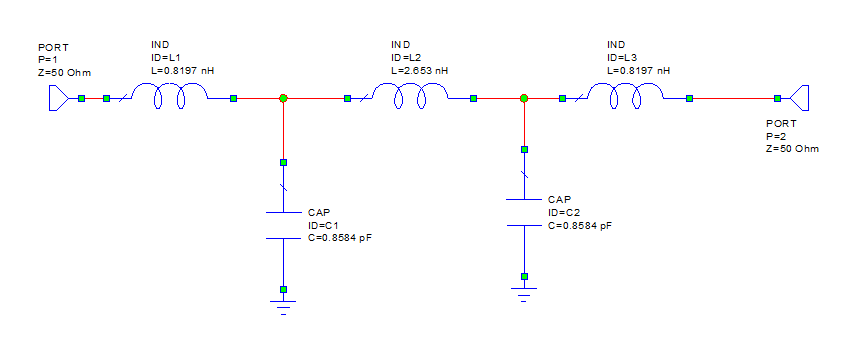
\includegraphics[scale=0.4]{lumped_schematic.png}
    \caption{5th order Butterworth Low Pass Filter implementation using lumped element components.}
    \label{fig:lumpedschematic}
\end{figure}

% Change the values given in this table
\begin{table}[!htbp]
\centering
\begin{tabular}{|l | c | c| c | c |}
    \hline
    $g_k$ & $L_k$ [nH] & $C_k$ [pF] & $l$ [mils] & $l$ optimized [mils] \\
    \hline
    1 & 0.8197 & - & 40.32 & 47 \\
    2 & - & 0.8584 & 105.97 & 95.5 \\
    3 & 2.653 & - & 130.43 & 107 \\
    4 & - & 0.8584 & 105.97 & 95.5 \\
    5 & 0.8197 & - & 40.32 & 47 \\
    \hline
\end{tabular}
    \caption{Design parameters of the 5th order Butterworth Filter. The lumped element series inductances and shunt capacitances have been given in addition to the line widths for the stepped filter implementation. }
    \label{tab:parameters}
\end{table}

To translate from lumped element to a stepped implementation of the filter, we noted that short sections of transmission lines with characteristic impedances $Z_{HI}$ and $Z_{LO}$ chosen such that $Z_{HI} \gg Z_0$ and $Z_{LO} \ll Z_0$ can be used as inductors and capacitors respectively. We chose the impedances of the transmission lines by choosing the width of the microstrip line. For $Z_{HI} = 97.57 \Omega$, we used 6 mil wide microstrip, while for $Z_{LO} = 29.73 \Omega$, we used 120 mil wide microstrip lines. With the choice of impedance fixed, the value of the inductance or capacitance is determined by the electrical length $\beta l$ of the microstrip section. For the inductive case, $\beta l = g_k Z_0 /Z_{HI}$ and for the capacitive case $\beta l = g_k Z_{LO}/Z_0 $. Using the TX Line tool in MWO, we were able to calculate the physical length of the microstrip lines once the electrical length was specified using the equations given. These values have also been given in table \ref{tab:parameters}. 

% \ref{fig:steppedschematic}

A circuit schematic was assembled in MWO as shown in figure \ref{fig:steppedschematic}  . To better model the physical circuit, we used the microstrip MSTEP elements, based on electromagnetic (EM) simulations, to capture the discontinuity in line width in moving from high impedance to low impedance sections of the filters. The circuit was simulated and we optimized the circuit to achieve cutoff at exactly 6 GHz. Since odd order Butterworth filters are symmetric about their midplane, we tune only 3 line lengths for the 5 element filters. Figure \ref{fig:lumpedvsstepped} shows a comparison of the simulation results between a stepped and a lumped element fifth order filter. Both filters show very similar responses in their passband and with similar cutoffs. However, the roll-off for the stepped implementation is much shallower than the lumped element case. This is because the stepped filter does not attenuate signals at arbitrarily high frequencies. Infact, the filter response repeats as a series of passbands and attenuated bands as you move to higher frequencies. 

\begin{figure*}[!htbp]
    \centering
    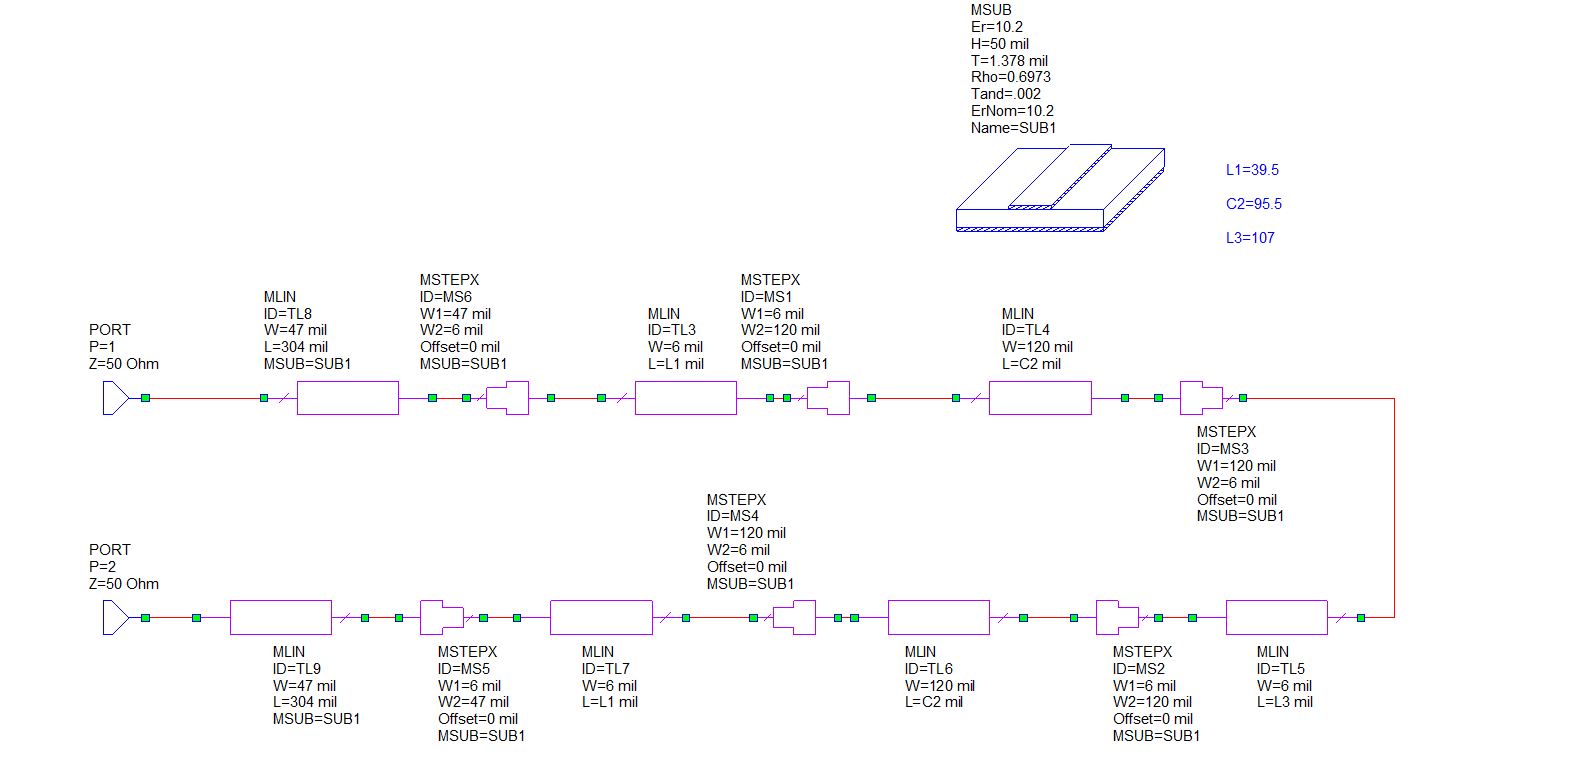
\includegraphics[scale=0.4]{stepped_schematic.png}
    \caption{5th order Butterworth Low Pass Filter implementation using transmission line sections.}
    \label{fig:steppedschematic}
\end{figure*}
%Need to include figures for the lumped element and stepped filter circuit schematics.

\begin{figure}[!htbp]
    \centering
    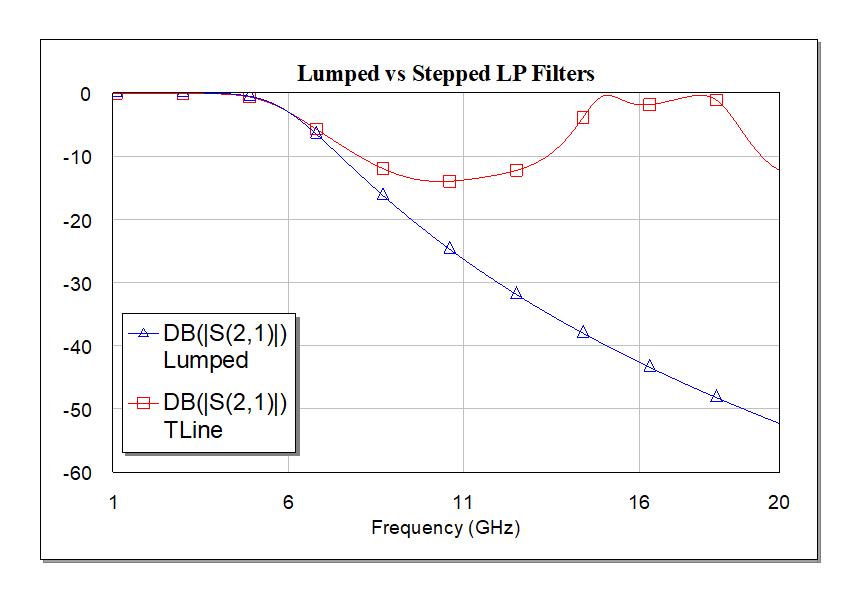
\includegraphics[scale=0.4]{lumped_vs_stepped.png}
    \caption{A comparison between the lumped and stepped implementation of the Butterworth filters. The stepped implementation has a higher passband starting at about 14 GHz.}
    \label{fig:lumpedvsstepped}
\end{figure}

\section*{Amplifier Design}\label{sec:ampdesign}
The goal of the amplifier design was to maximize the transducer gain, $G_T$ of the amplifier. The transducer gain is defined as the ratio of the power delivered to the load to the available power from the source. The power delivered to the load with a reflection coefficient, $\Gamma_l$ by the two port network of the amplifier is given by $P_{del} = |b_2|^2 \left(1 - |\Gamma_l|^2\right) $. The power available from the source with source power $|a_s|^2$ and a reflection coefficient $\Gamma_s$ is given by $P_{avs} = |a_s|^2 /\left(1 - |\Gamma_s|^2 \right)$. Combining these two expressions and using Mason's rule to find $b_2$, we can reexpress the transducer gain as 

\begin{equation}
    G_T = \frac{1 - |\Gamma_s|^2}{|1 - \Gamma_s \Gamma_{in}|^2} \cdot |S_{21}|^2 \cdot \frac{1  - |\Gamma_l|^2}{|1 - \Gamma_l S_{22}|^2}
    \label{eqn:transducergain}
\end{equation}

Here, $\Gamma_{in} = S_{11} + \frac{S_{21} \Gamma_l S_{12}}{1 - S_{22} \Gamma_l}$ is the input impedance of the amplifier with the load connected to it. From equation \ref{eqn:transducergain}, we can conclude that in order to maximize the gain, two conditions must be satisfied; $\Gamma_s = \Gamma_{in}^*$ and $\Gamma_l = S_{22}^*$ in addition to making $|S_{21}|$ as large as possible. The value of $S_{21}$ is a function of the biasing conditions of the amplifier. As a result, we maximized it by choosing the transistor bias of 2 V with 20 mA current at the output of the transistor network. The biasing circuit used for the transistor is shown in figure \ref{fig:ampbiasschematic}. 

\begin{figure*}[!htbp]
    \centering
    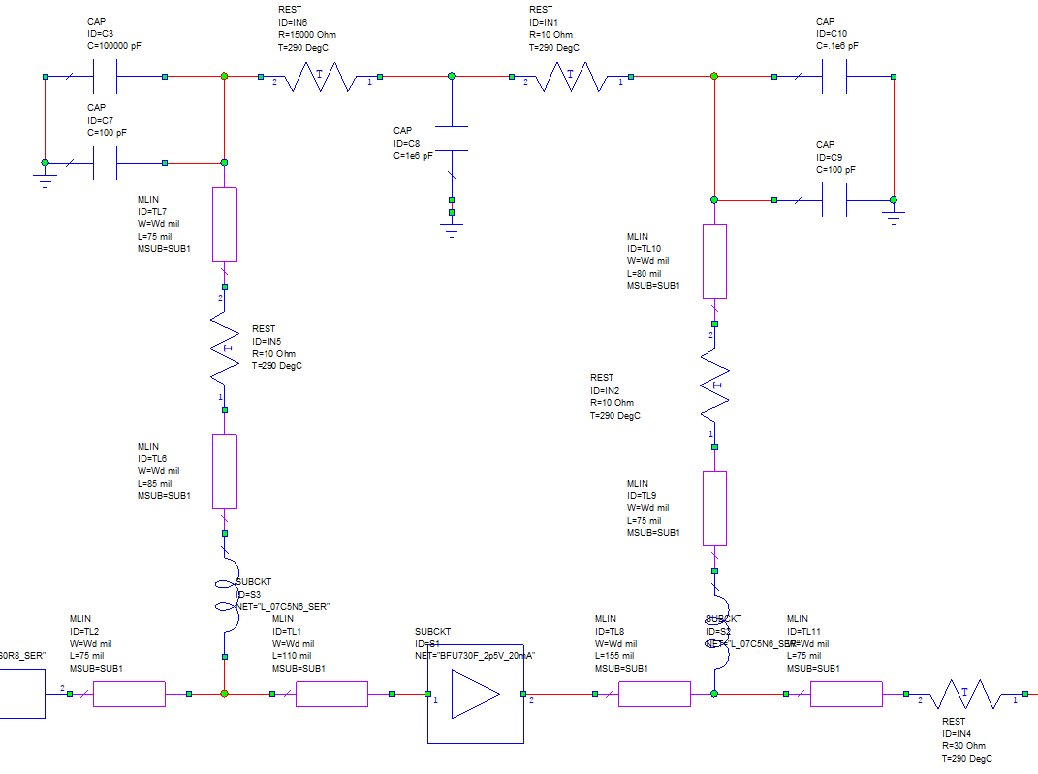
\includegraphics[scale=0.4]{Biasing_Network.png}
    \caption{The biasing network chosen to achieve 2 V at the output with 20 mA collector current. The inductors in the biasing network are used for amplifier stability.}
    \label{fig:ampbiasschematic}
\end{figure*}

With the bias chosen, we then designed a matching network at the transistor output to transform the $50 \Omega$ load to one that satisfies $\Gamma_l = S_{22}^*$. We designed the matching network using lumped element capacitors and inductors. For the output matching, a single 1 nH inductor sufficed to give a -12.24 dB match at 6 GHz. The output matching network is shown in figure \ref{fig:outputmatch} and the level of match achieved is shown in figure FIX THIS.


\begin{figure}[!htbp]
    \centering
    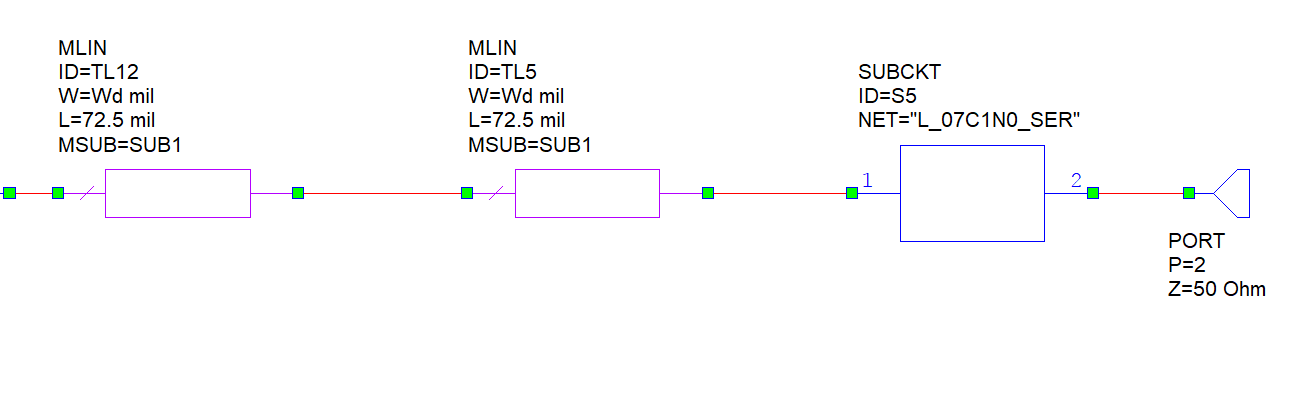
\includegraphics[width=0.5\textwidth]{output_matching_network.png}
    \caption{Output matching network for the power amplifier.}
    \label{fig:outputmatch}
\end{figure}


The output matching network fixes $\Gamma_l$ which sets the value of $\Gamma_{in}$ for the input matching network. We again designed the input matching network using a combination of series capacitors and shunt inductors as shown in figure \ref{fig:inputmatch}. We achieved a -20.1 dB input match as shown in figure \ref{fig:inputoutputmatching}

\begin{figure}[!htbp]
    \centering
    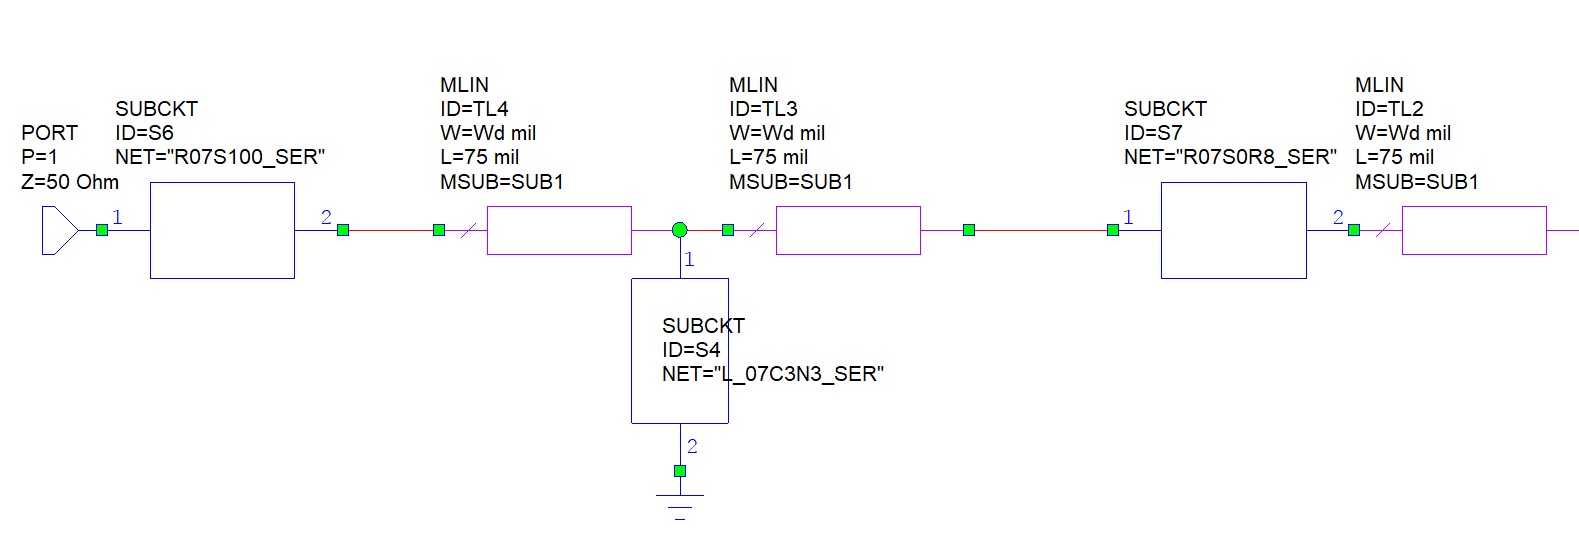
\includegraphics[width=0.5\textwidth]{input_matching_network.png}
    \caption{Input matching network for the power amplifier.}
    \label{fig:inputmatch}
\end{figure}



\begin{figure}[!htbp]
    \centering
    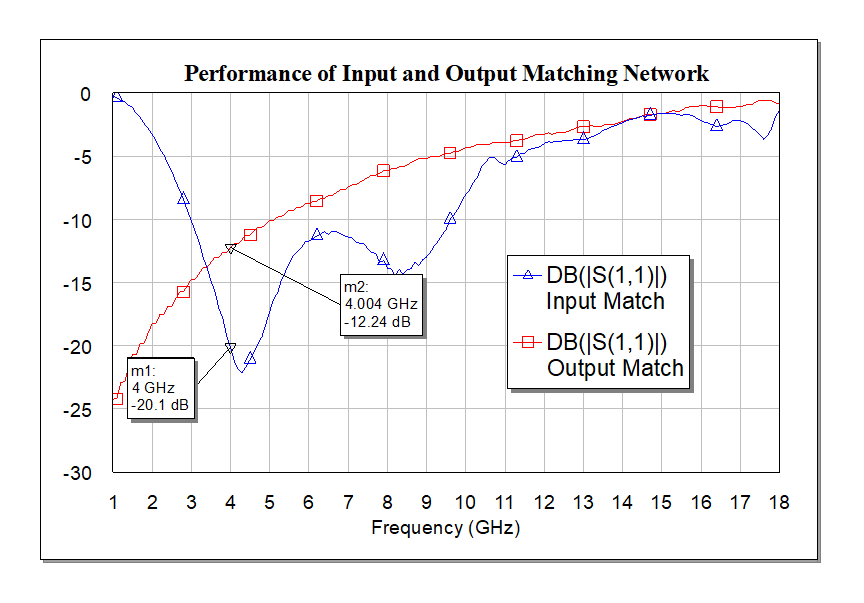
\includegraphics[width=0.5\textwidth]{input_and_output_matching.png}
    \caption{Input and Output network matching performance for the power amplifier.}
    \label{fig:inputoutputmatching}
\end{figure}

With the choice of input and output matching networks, we expected to achieve a transducer gain of 16 dB at 6 GHz as shown in figure \ref{fig:ampgain}.

\begin{figure}[!htbp]
    \centering
    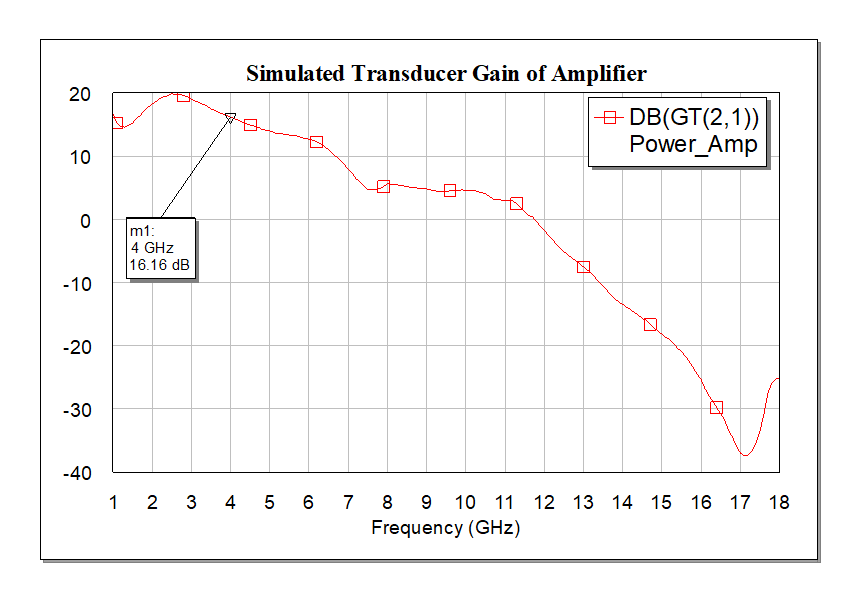
\includegraphics[width=0.5\textwidth]{amplifier_gain.png}
    \caption{Simulated transducer gain of amplifier.}
    \label{fig:ampgain}
\end{figure}

\section*{Lab Testing}\label{sec:testing}

At the start of the lab session, we deburred the low pass filter microstrip circuit and soldered on its SMA connectors. The completed filter circuit is shown in figure \ref{fig:LPcloseup} In addition, based on the design of the bias and matching networks for the power amplifier, we replaced some of the lumped components from our lab 3 amplifier to complete our power amplifier.

\begin{figure}[!htbp]
    \centering
    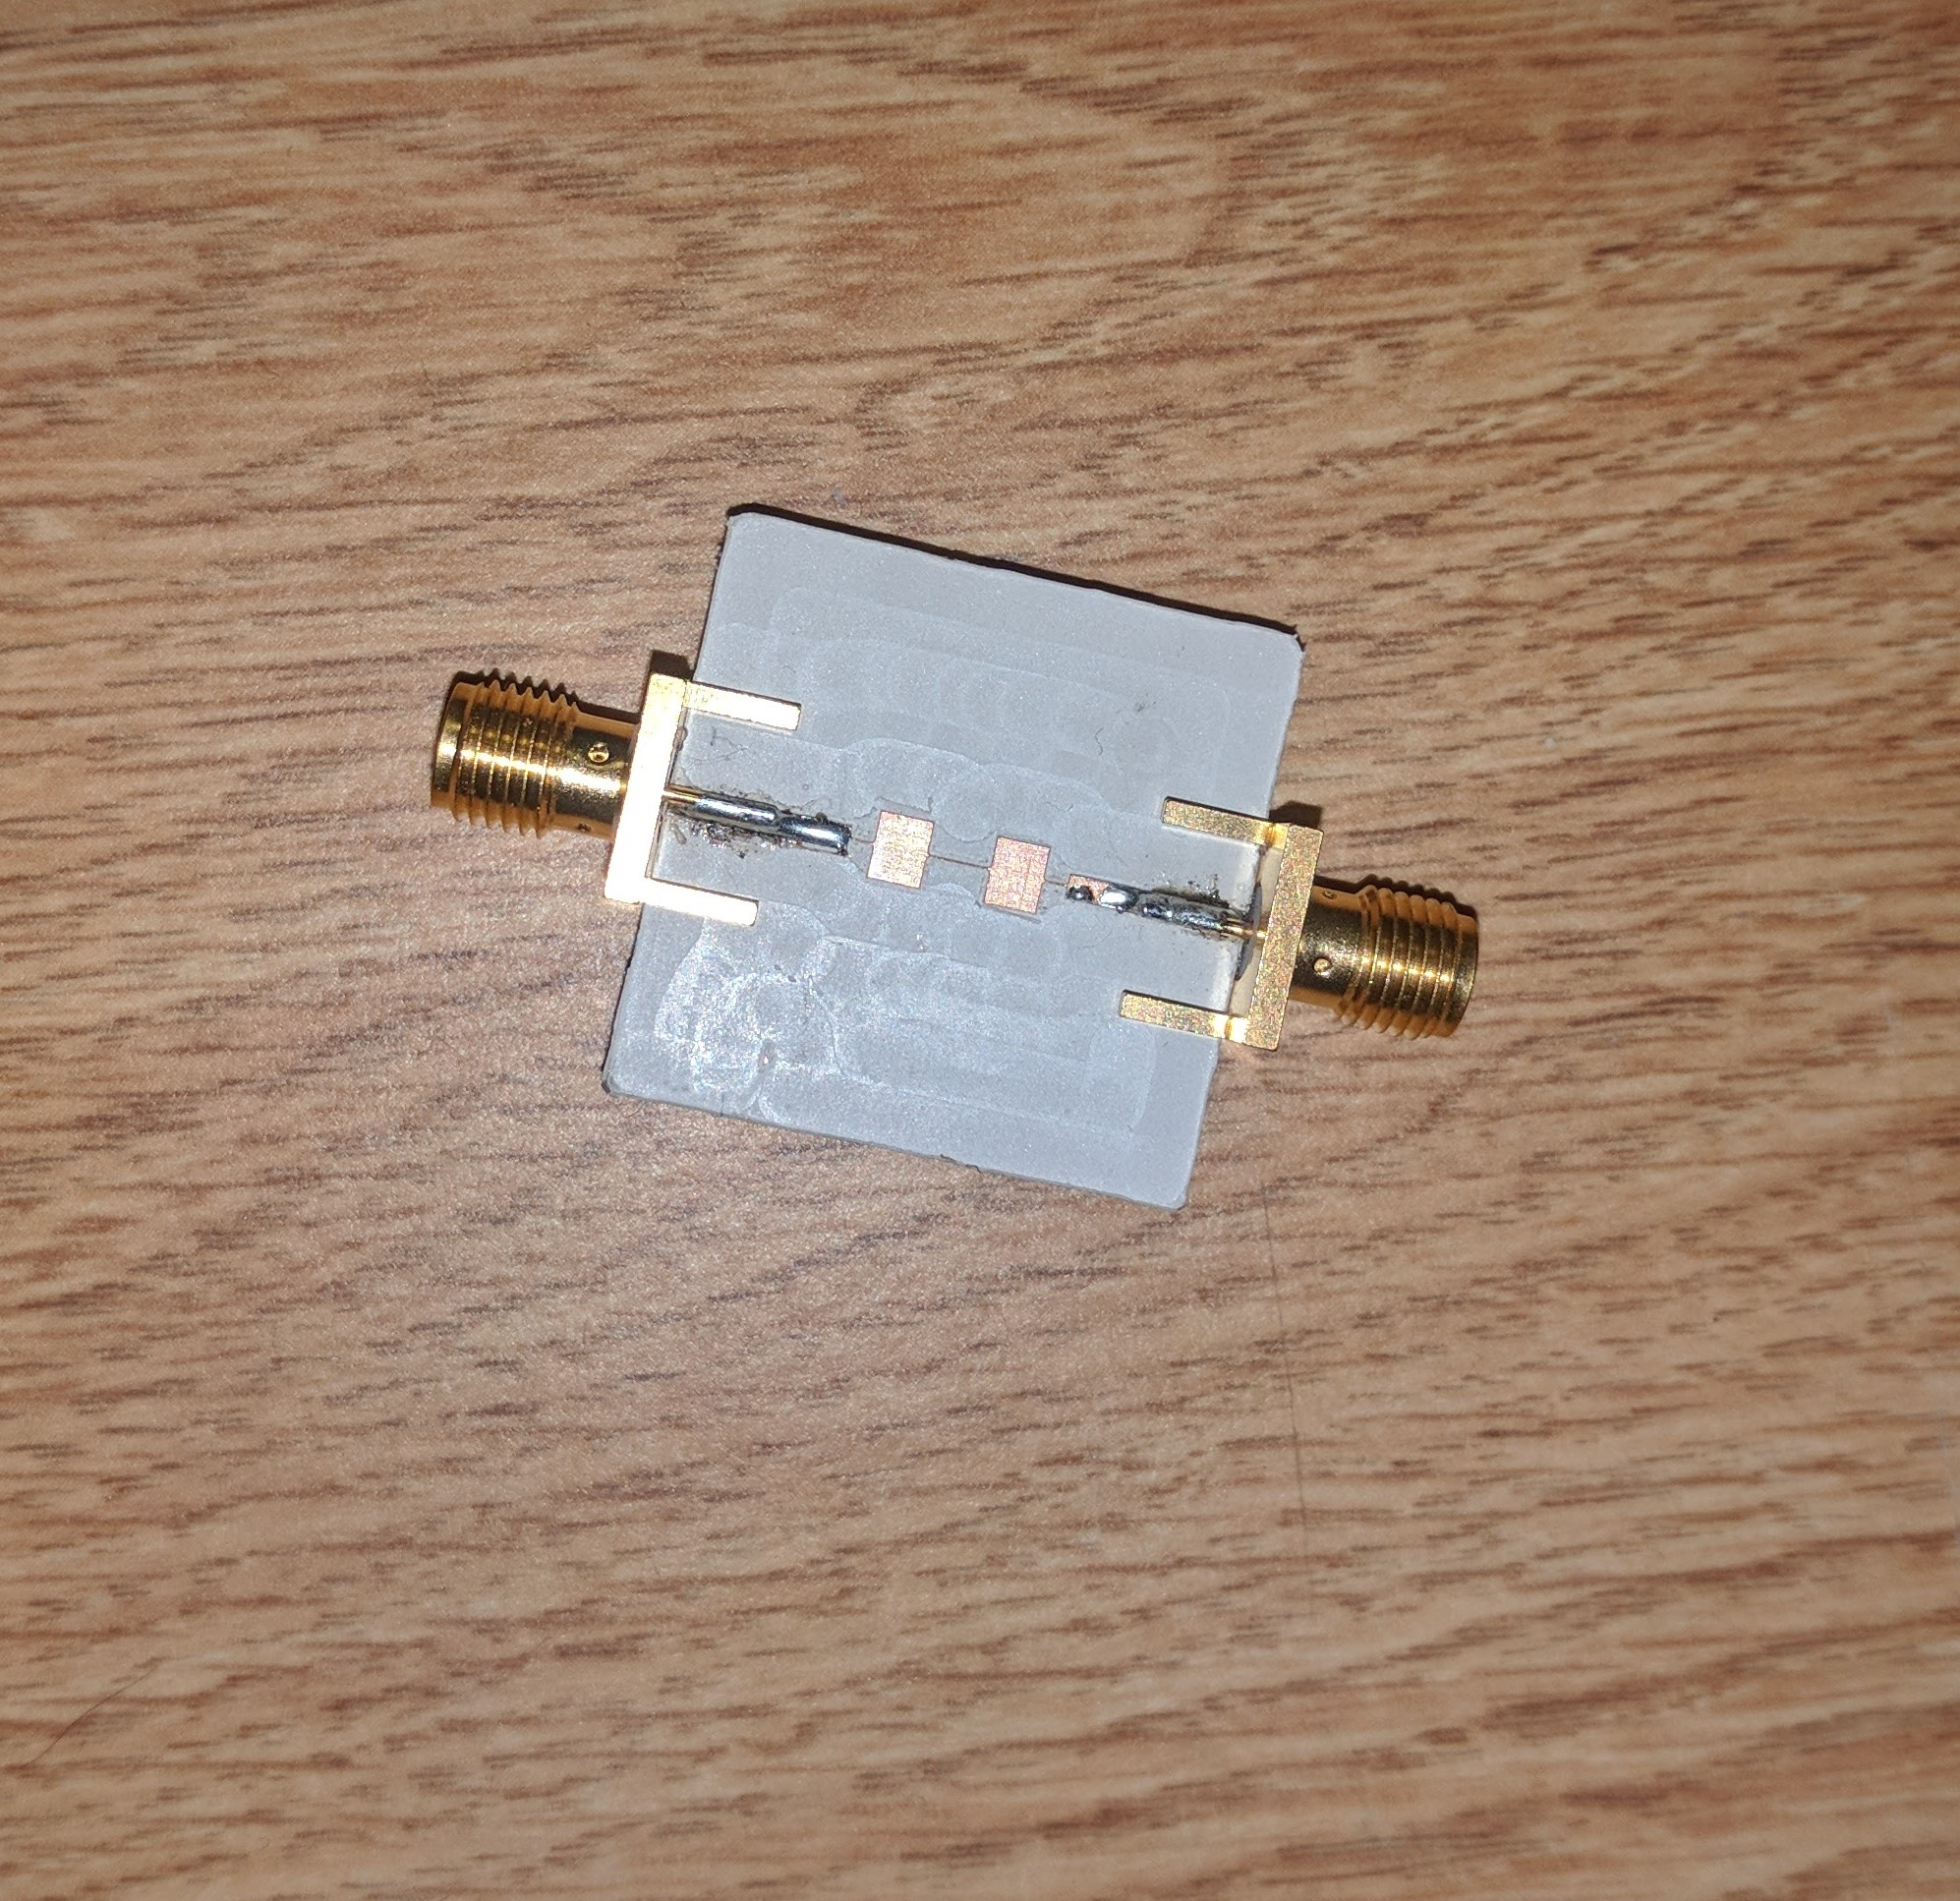
\includegraphics[width=0.5\textwidth]{LP_filter.jpg}
    \caption{Stepped LP filter with SMA connectors soldered on.}
    \label{fig:LPcloseup}
\end{figure}

The FFox was calibrated in NA mode to measure the S parameters of the LP filter over the frequency range 0.1-18 GHz. We set the output power to -5.0 dBm and saved the S parameters of the filter to file. An image of the measurement setup is shown in figure \ref{fig:LPsetup}. Once the filter measurements were completed, we recalibrated the FFox at a -30 dBm input power level to make measurements on the power amplifier over the same frequency range. The power supply for the amplifier was set with the OVP at 3.50 V and OCP at 0.01 A which was the minimum current setting on the power supply. We again measured the S parameters of the amplifier as shown in  figure \ref{fig:ampsetup}. The amplifier was biased at a 2.5 V at $V_{cc}$ and 20 mA current at the output as per the design. 

\begin{figure}[!htbp]
    \centering
    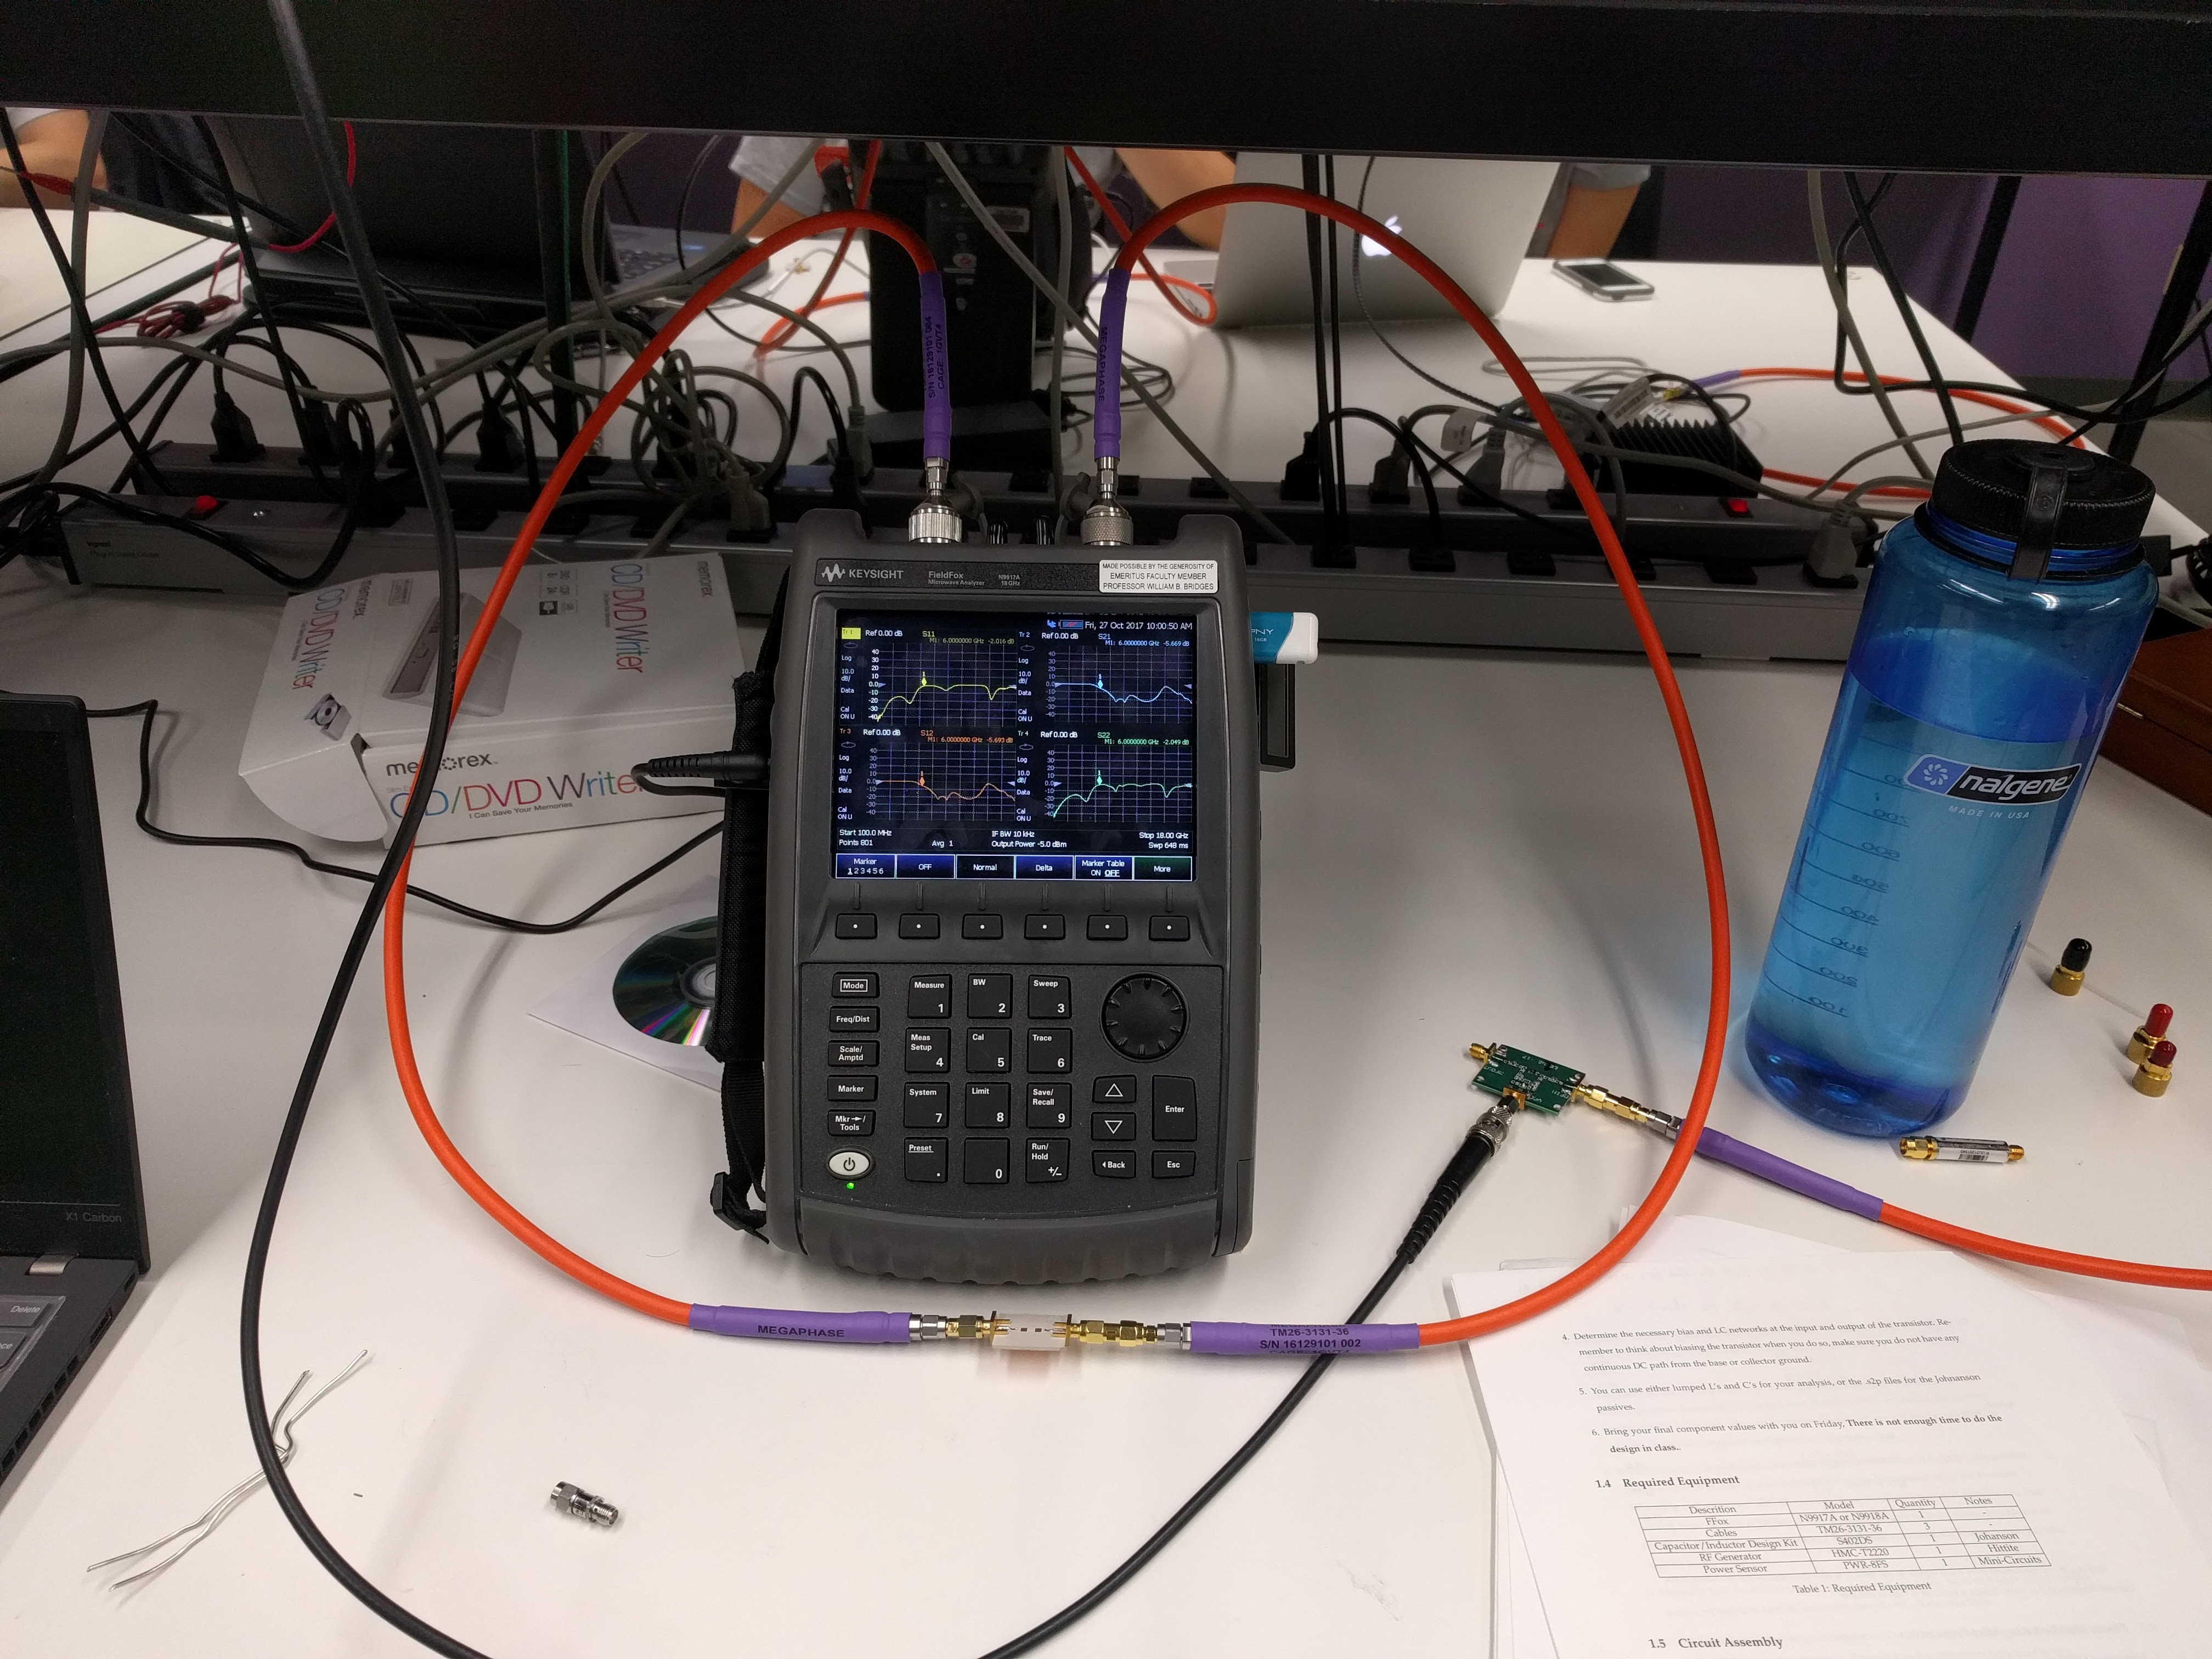
\includegraphics[width=0.5\textwidth]{LP_setup.jpg}
    \caption{FFox and LP filter setup for S parameter measurements.}
    \label{fig:LPsetup}
\end{figure}

\begin{figure}[!htbp]
    \centering
    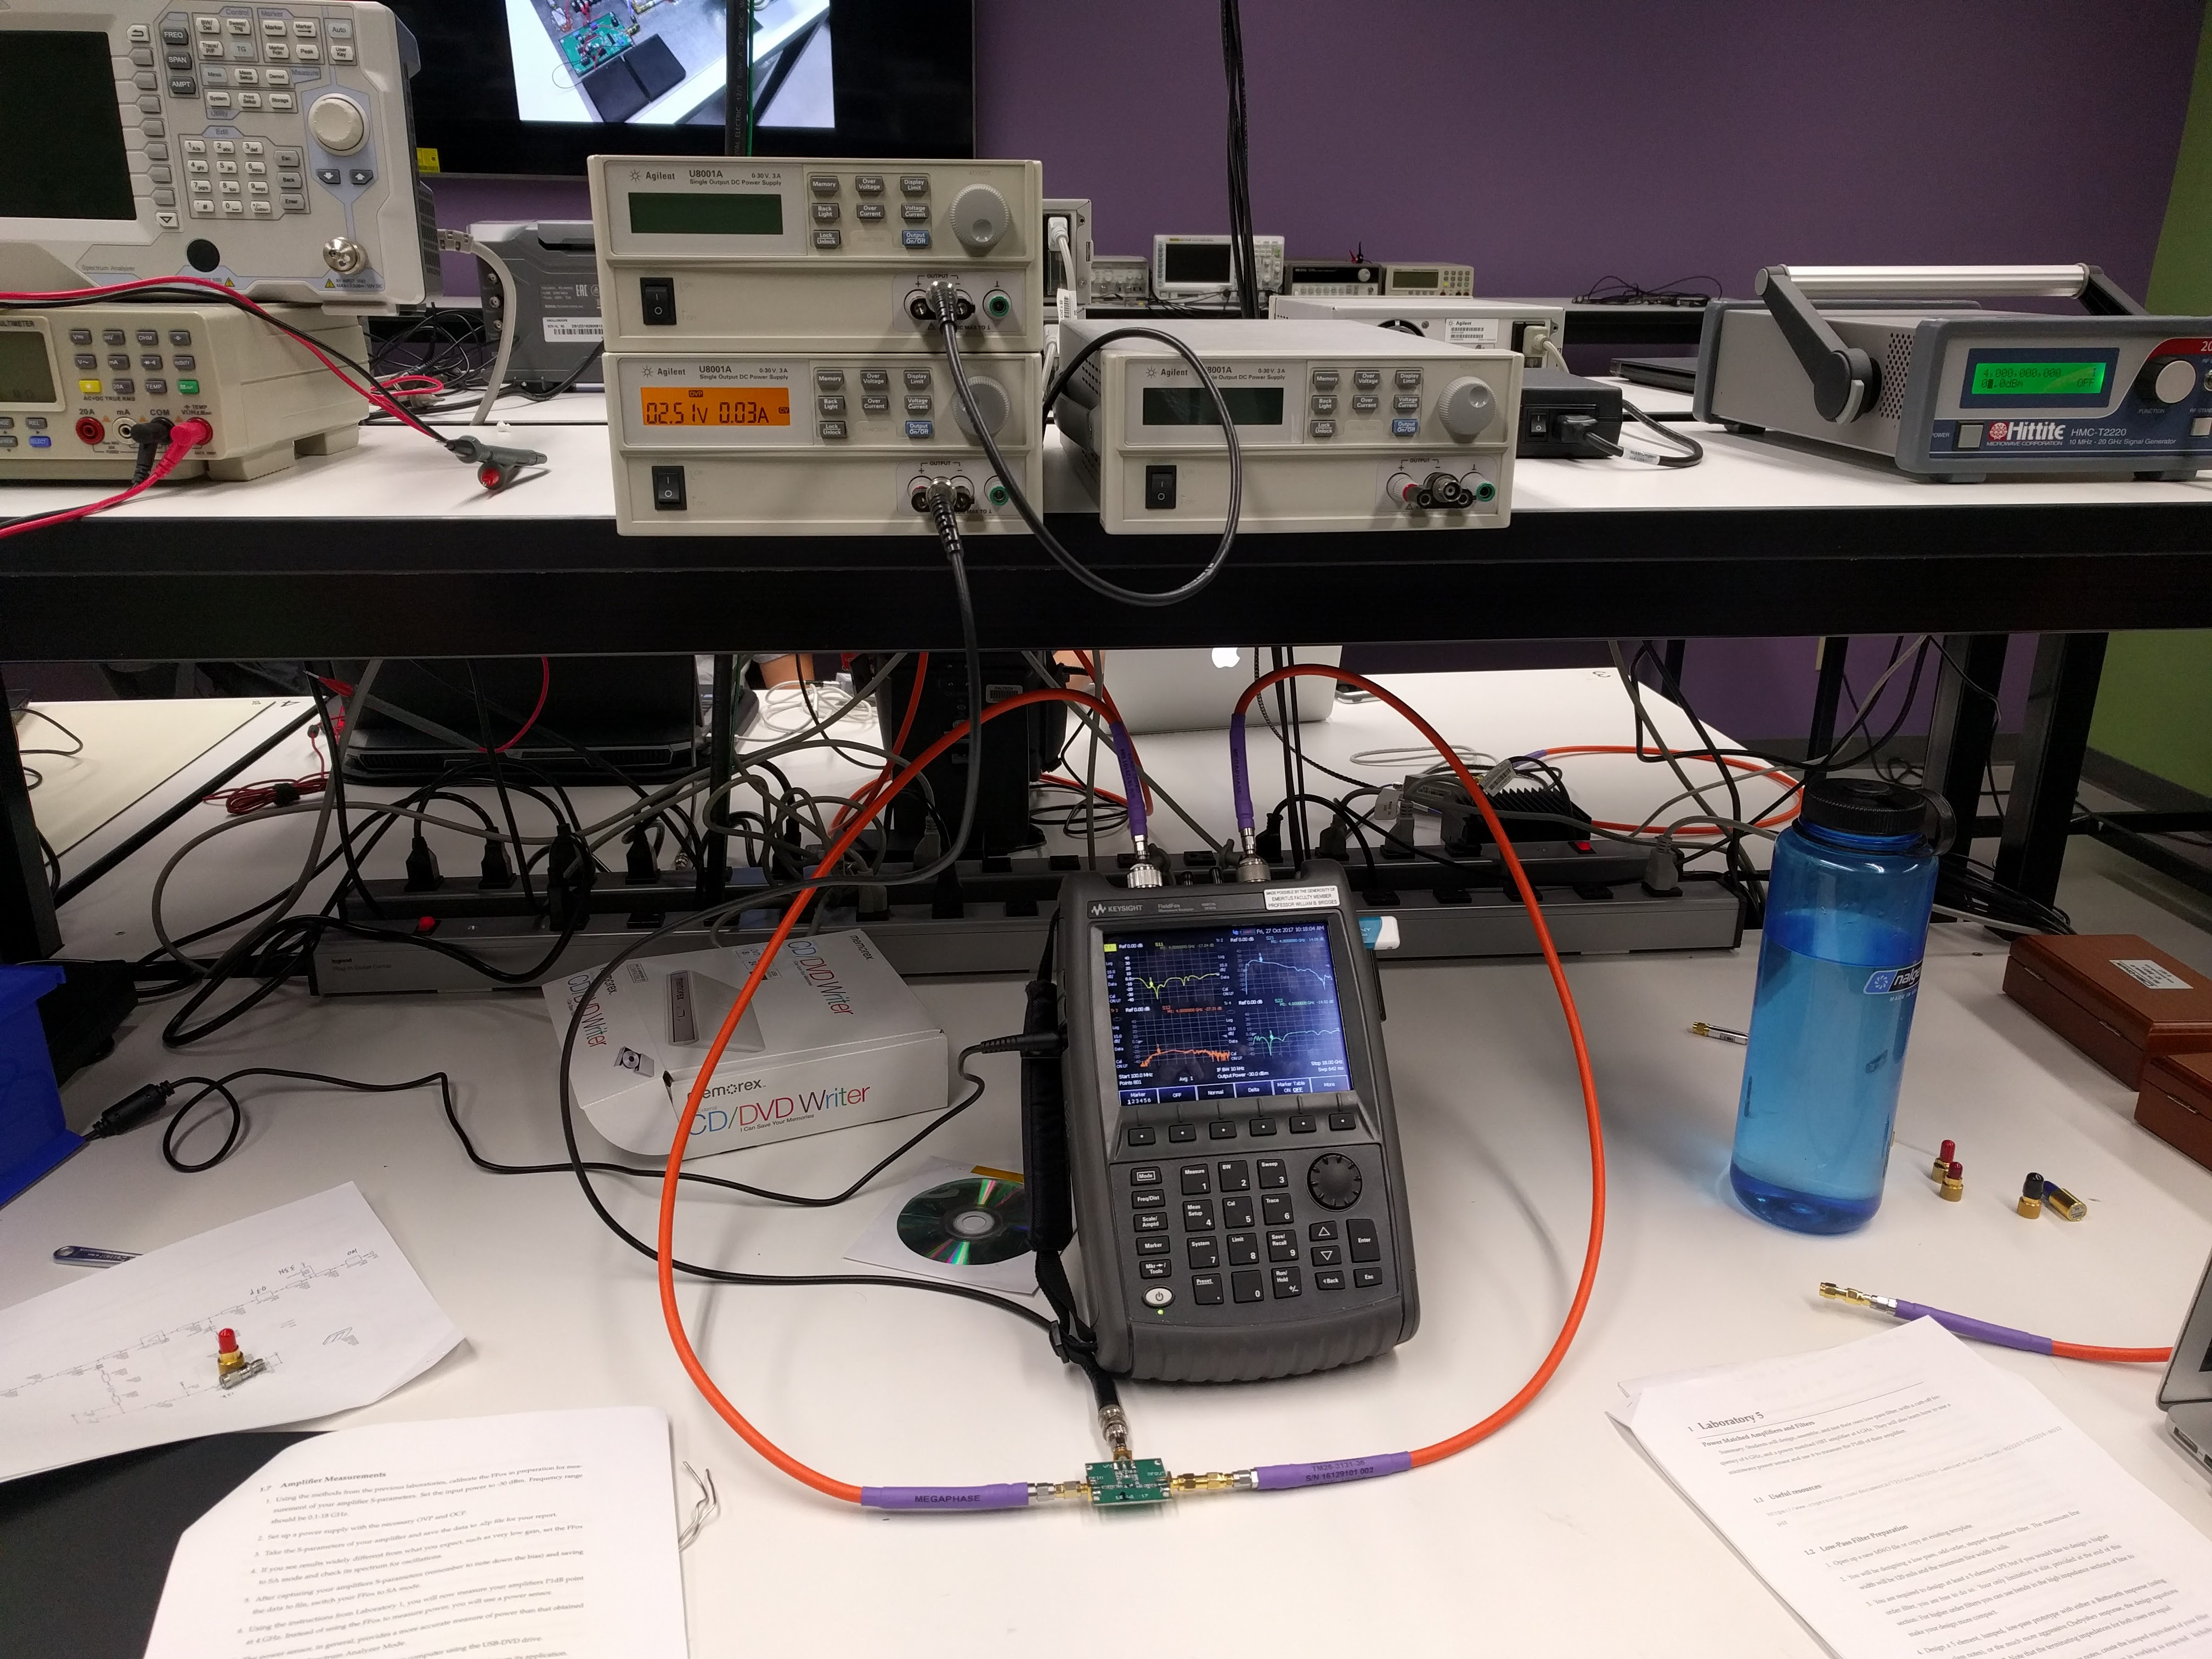
\includegraphics[width=0.5\textwidth]{amp_S_params2.jpg}
    \caption{FFox and power amplifier setup for S parameter measurements.}
    \label{fig:ampsetup}
\end{figure}

In order to measure the non-linearity in the response of the power amplifier, we changed the FFox mode to SA. We used a usb power sensor to measure the power output of the amplifier instead of directly using the FFox. This was because the power sensor gave much more accurate measurements of the power. We calibrated the power sensor against the hittite RF source at 4 GHz by stepping the Hittite power output from -20 dBm to 0 dBm and recording the power measured at the power sensor end. The calibration setup is shown in figure \ref{fig:powercalib}. 

\begin{figure}[!htbp]
    \centering
    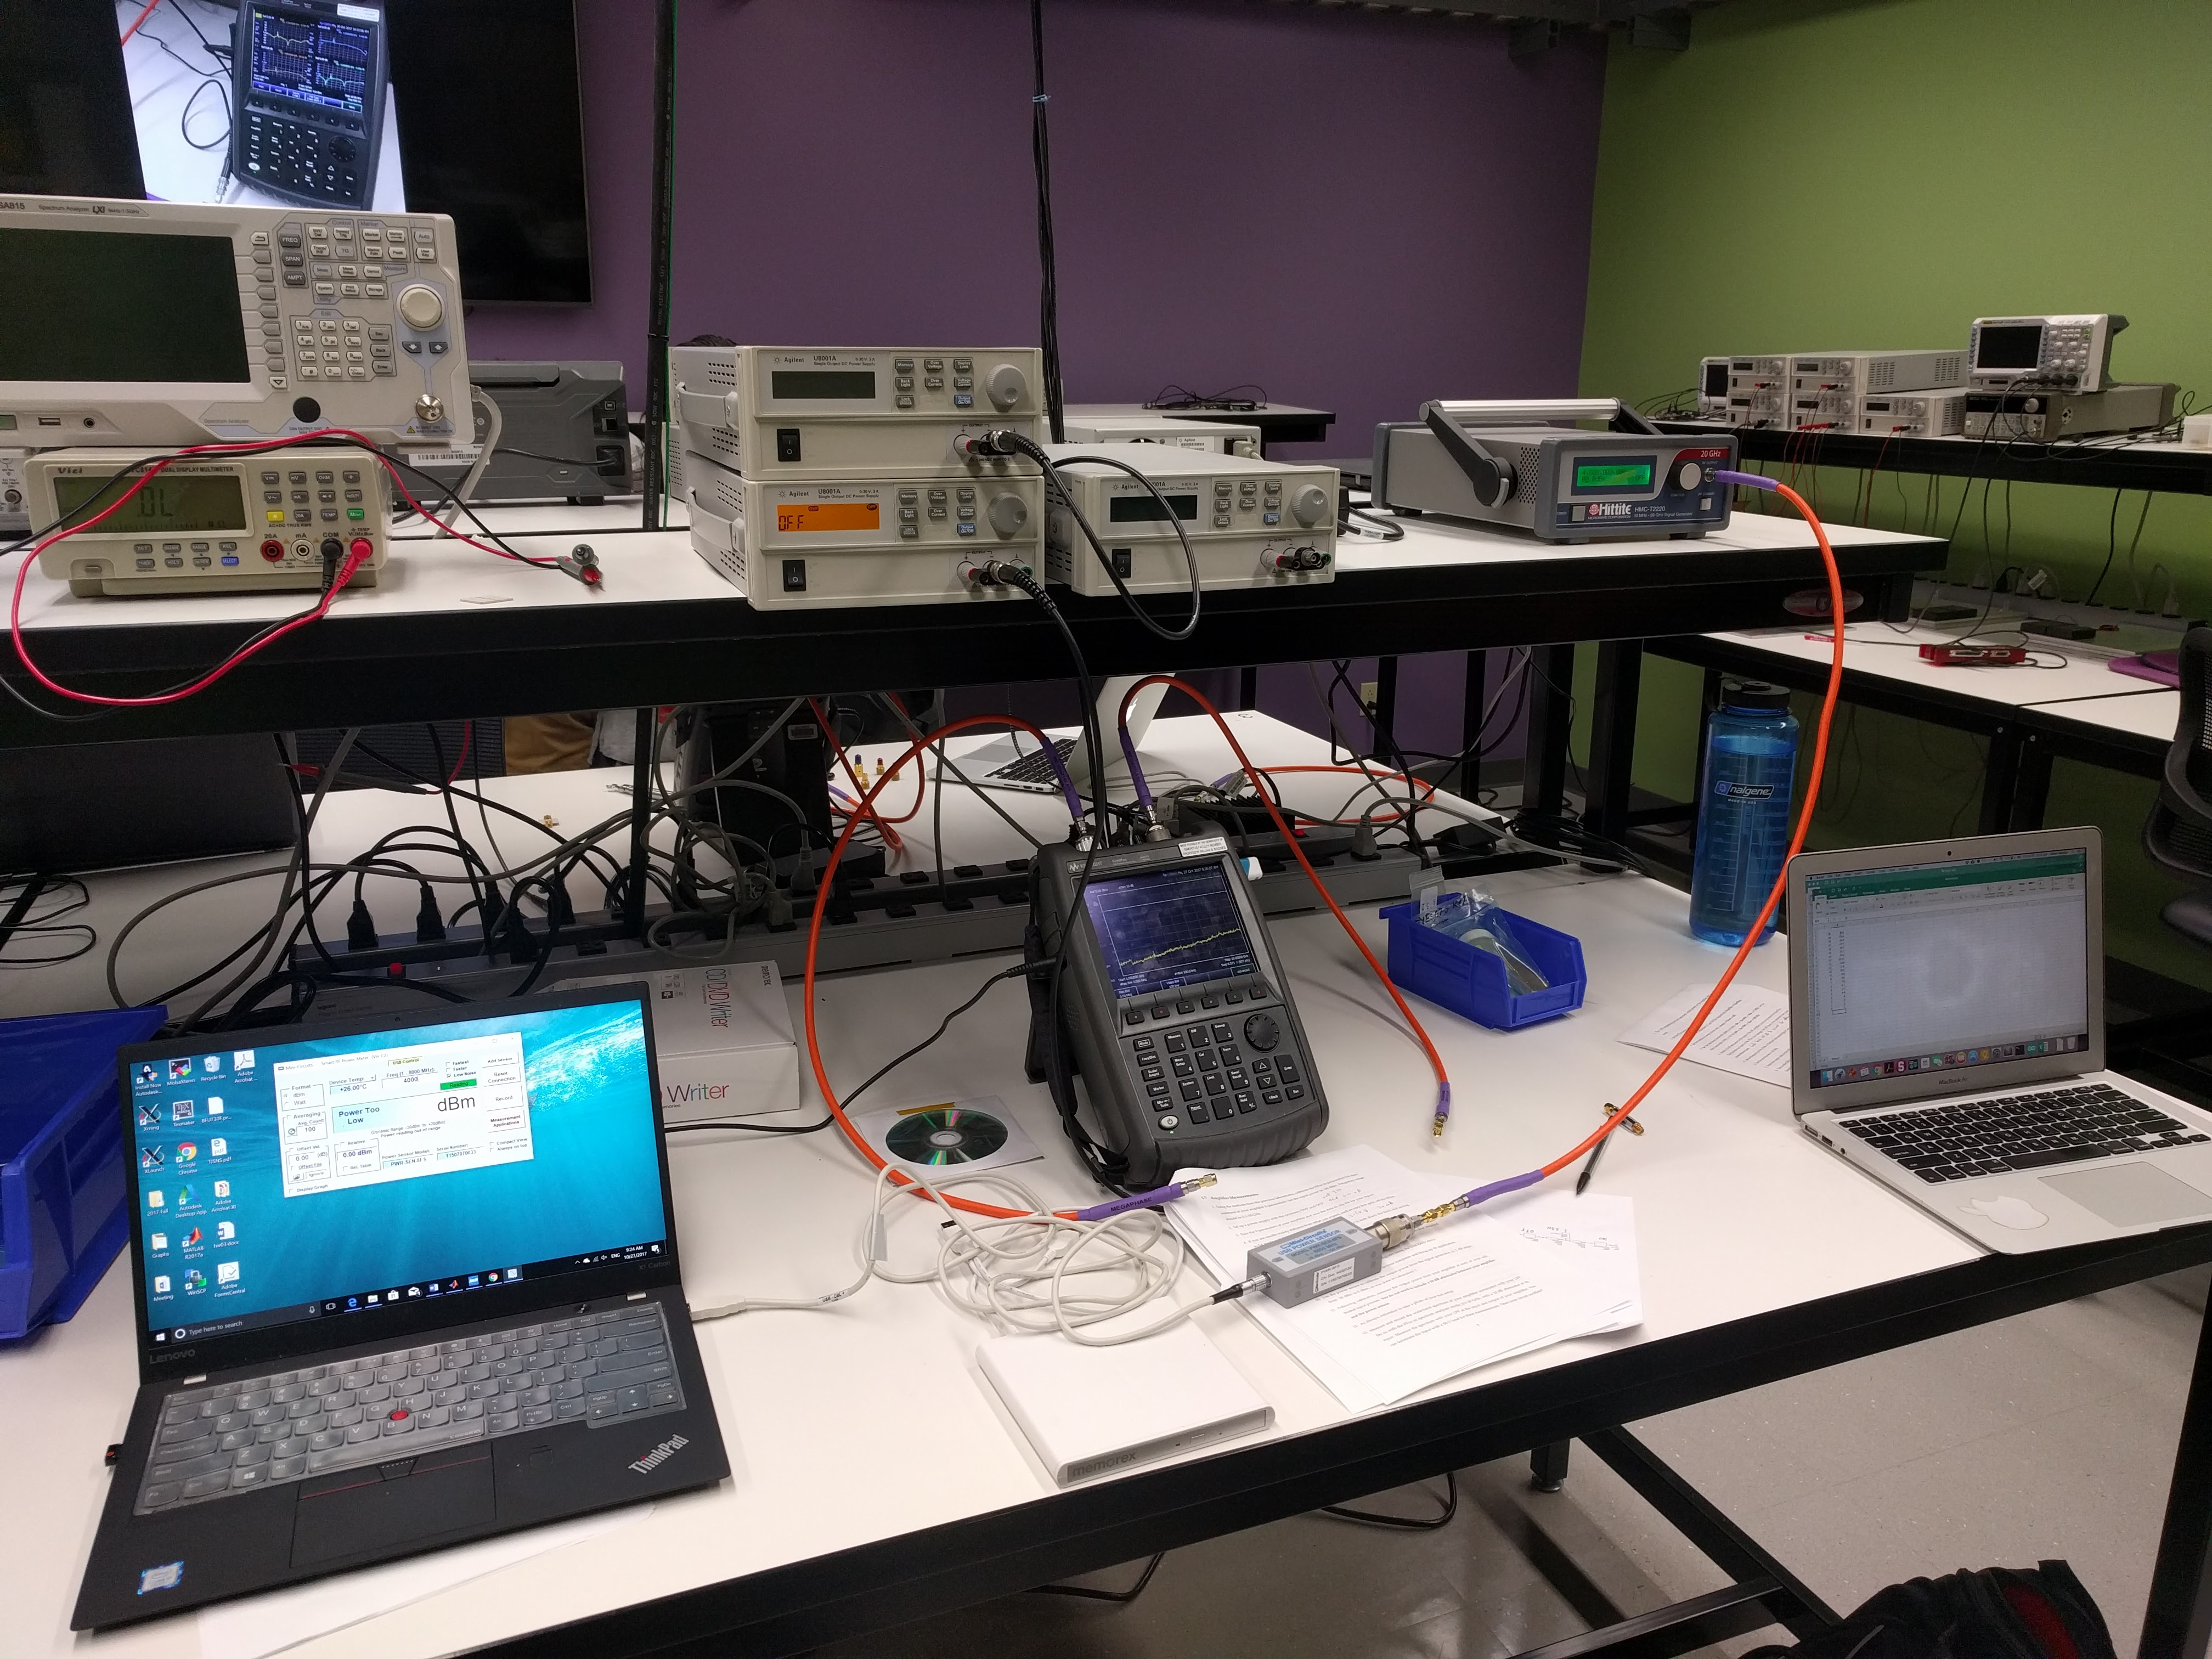
\includegraphics[width=0.5\textwidth]{power_sensor_calib.jpg}
    \caption{Setup for the power sensor calibration measurements.}
    \label{fig:powercalib}
\end{figure}

With the calibration completed, we measured the output power from the amplifier at each calibrated output power level of the Hittite RF source. Unlike with the FFox, we did not need to include any attenuators at the output of the amplifier to perform the measurements safely. The experimental setup for this measurement is shown in figure \ref{fig:ampSA}. 

\begin{figure}[!htbp]
    \centering
    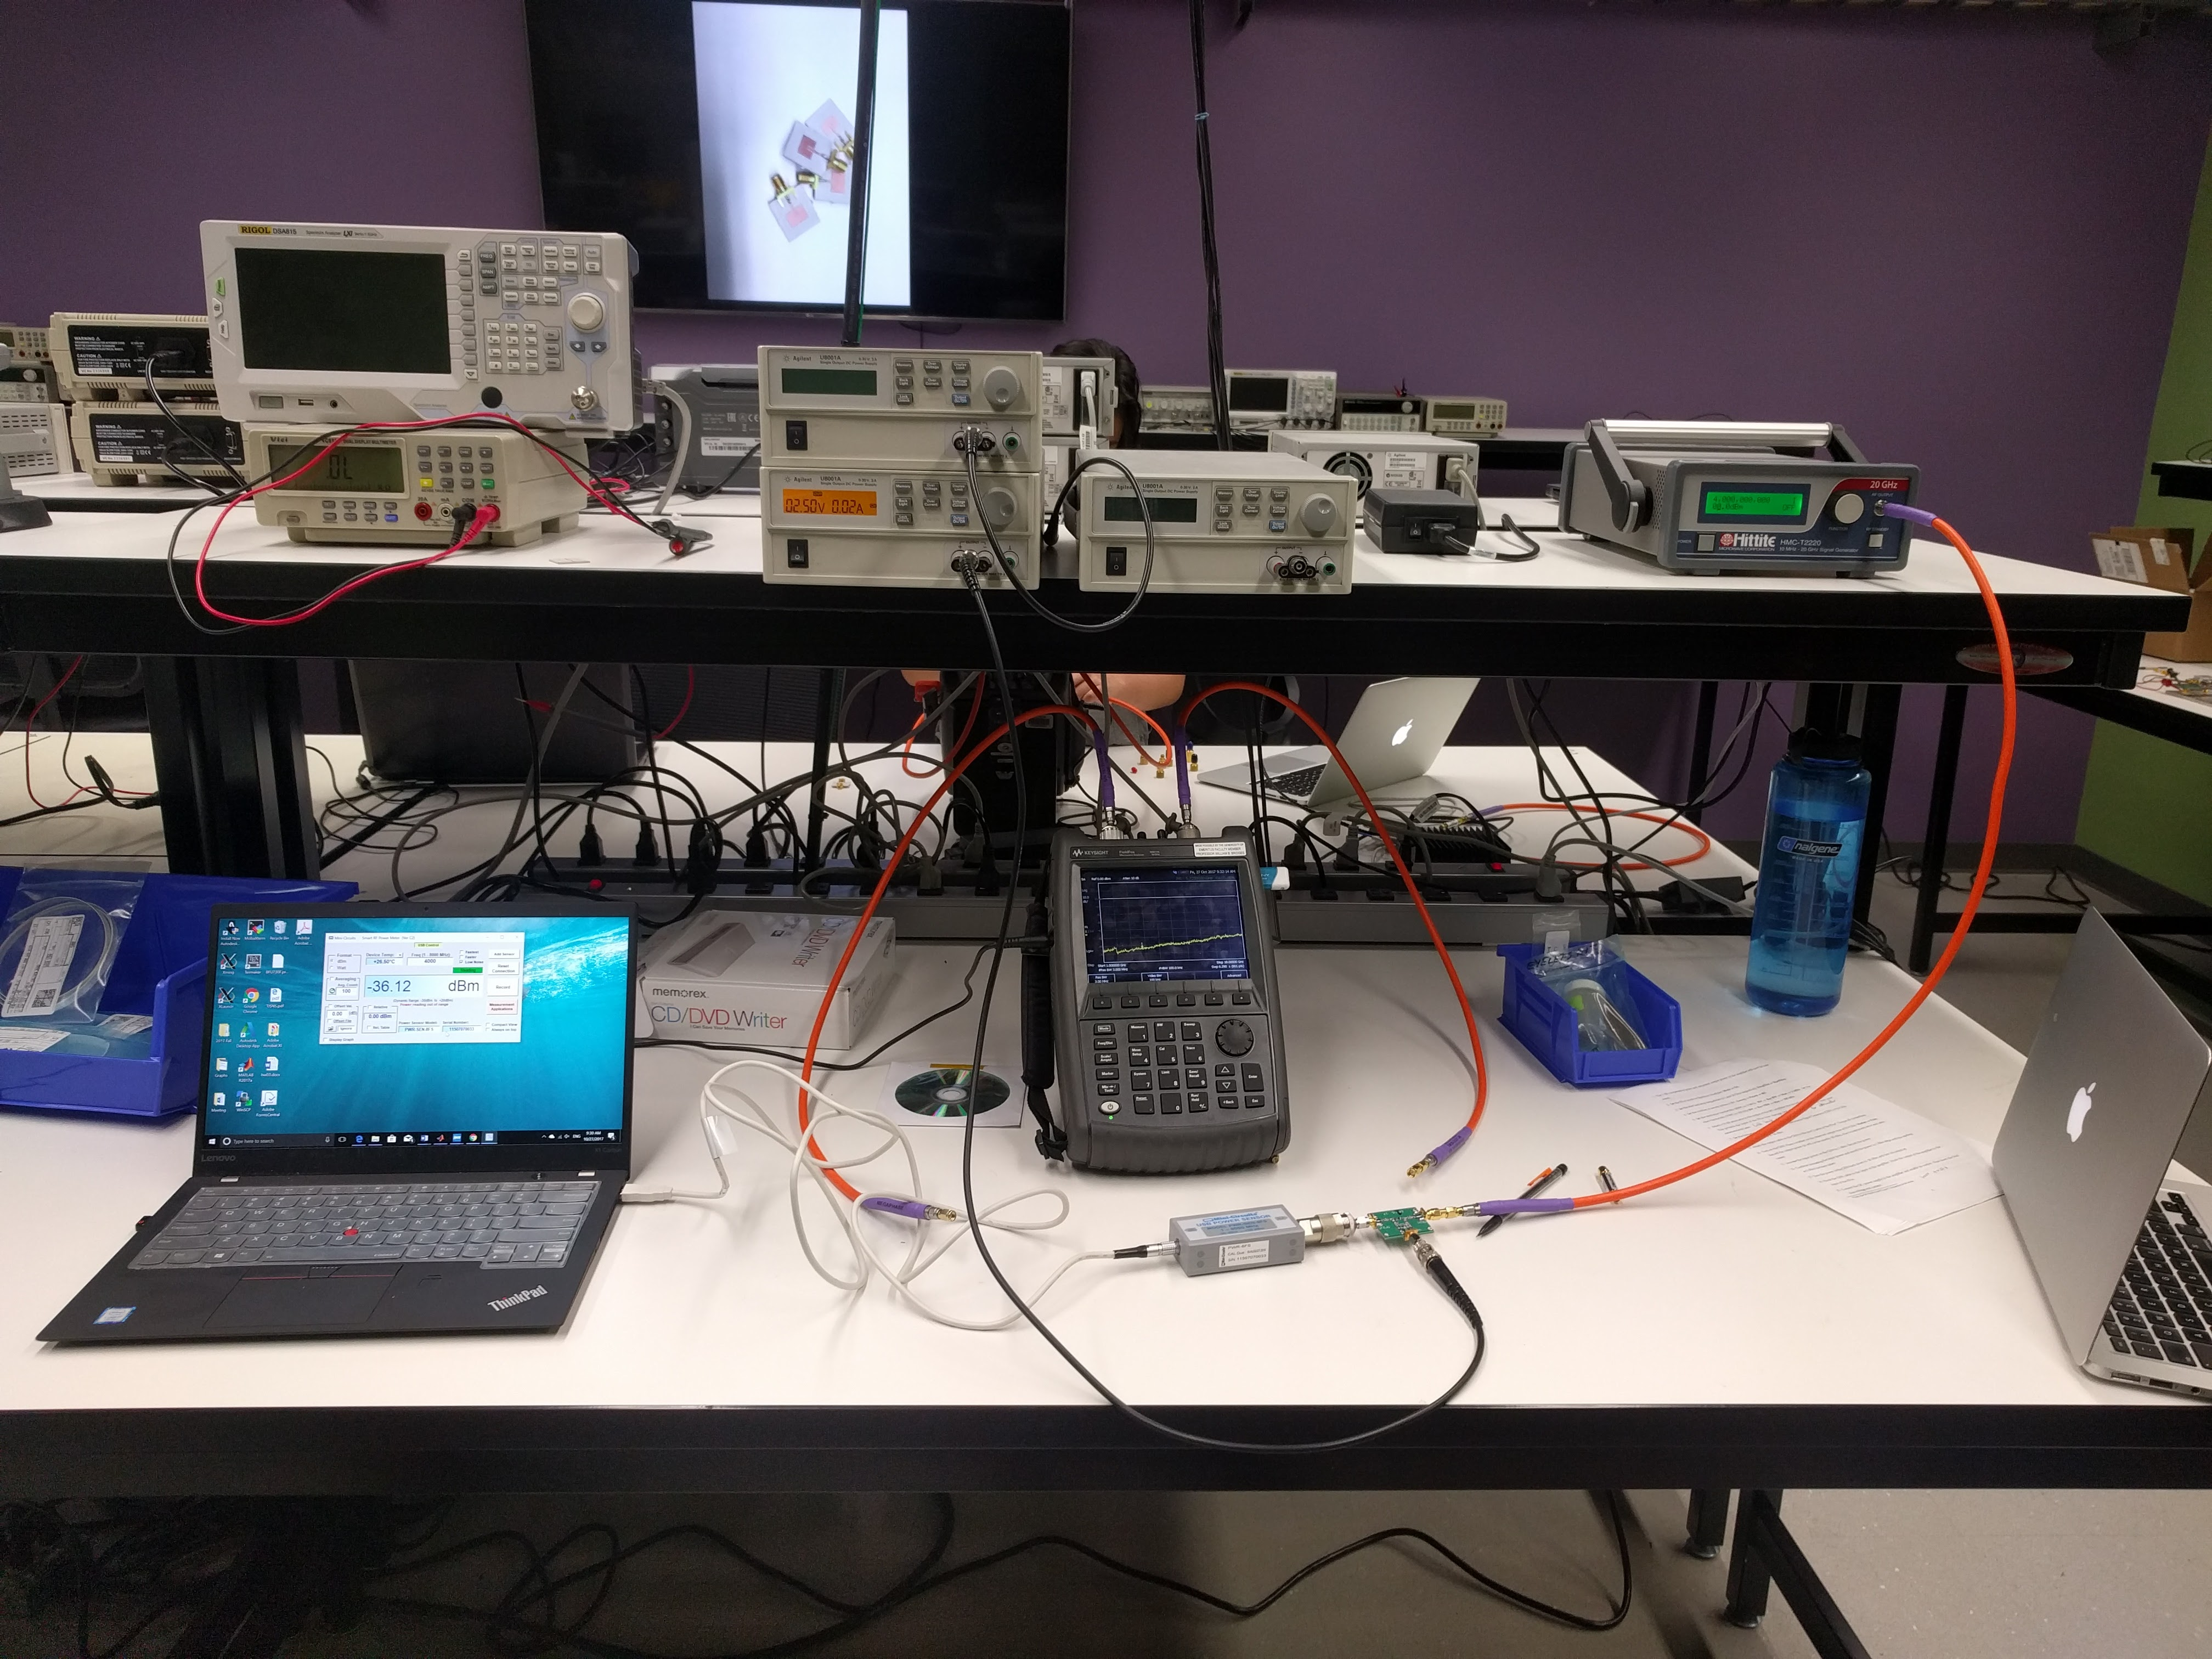
\includegraphics[width=0.5\textwidth]{amp_setup.jpg}
    \caption{Measurement of the 1 dB compression point of the amplifier using the power sensor and Hittite RF source.}
    \label{fig:ampSA}
\end{figure}

In addition, we tested the stability of the amplifier by connecting the input of the amplifier to the FFox and terminating the output with the low pass filter. We measured a wide band spectrum (0.1-18GHz) of the amplifier to check for any  peaks in the spectrum that may indicate that the amplifier was unstable. In this case, a 10 dB attenuator was used at the input of the FFox. We repeated the measurement with the filter at the input of the amplifier and again checked for peaks in the spectrum. We did not record any oscillations in these measurements. The setup with the filter at the input and at the output are shown in figures \ref{fig:ampLPinput}, \ref{fig:ampLPoutput} respectively.

\begin{figure}[!htbp]
    \centering
    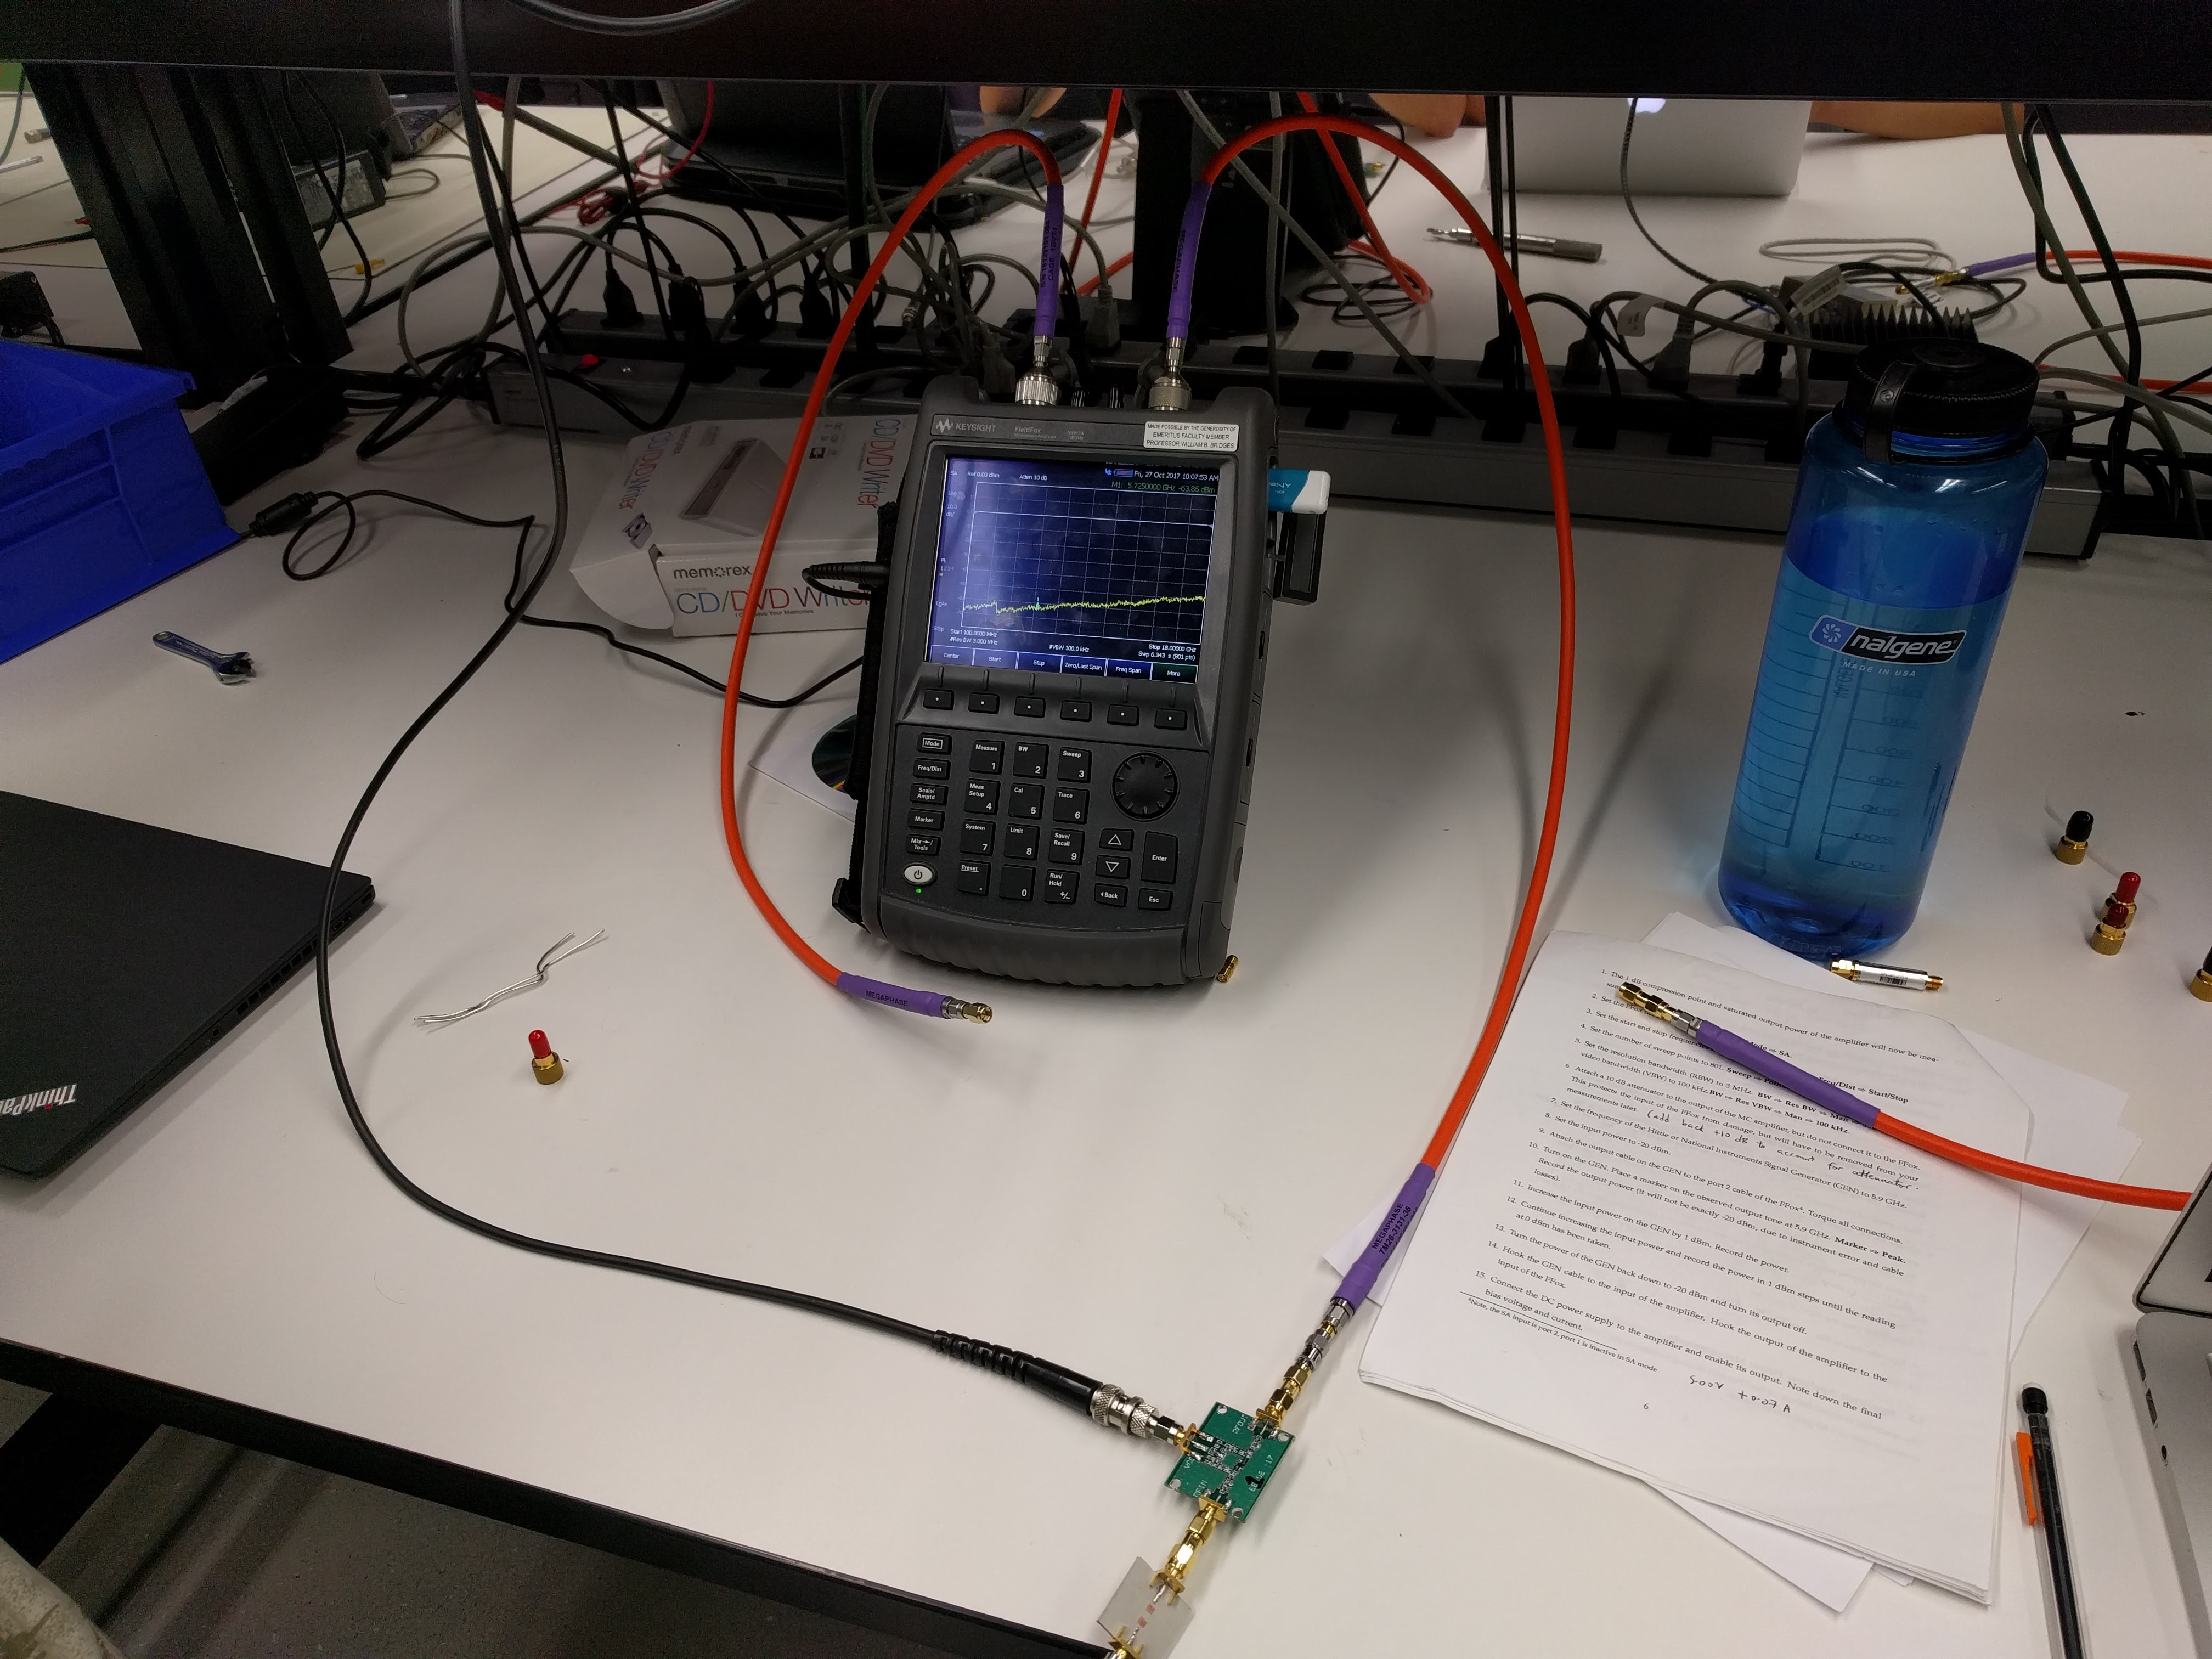
\includegraphics[width=0.5\textwidth]{amp_LP_input.jpg}
    \caption{Stability measurement of the amplifier with the LP filter at the input of the amplifier.}
    \label{fig:ampLPinput}
\end{figure}

\begin{figure}[!htbp]
    \centering
    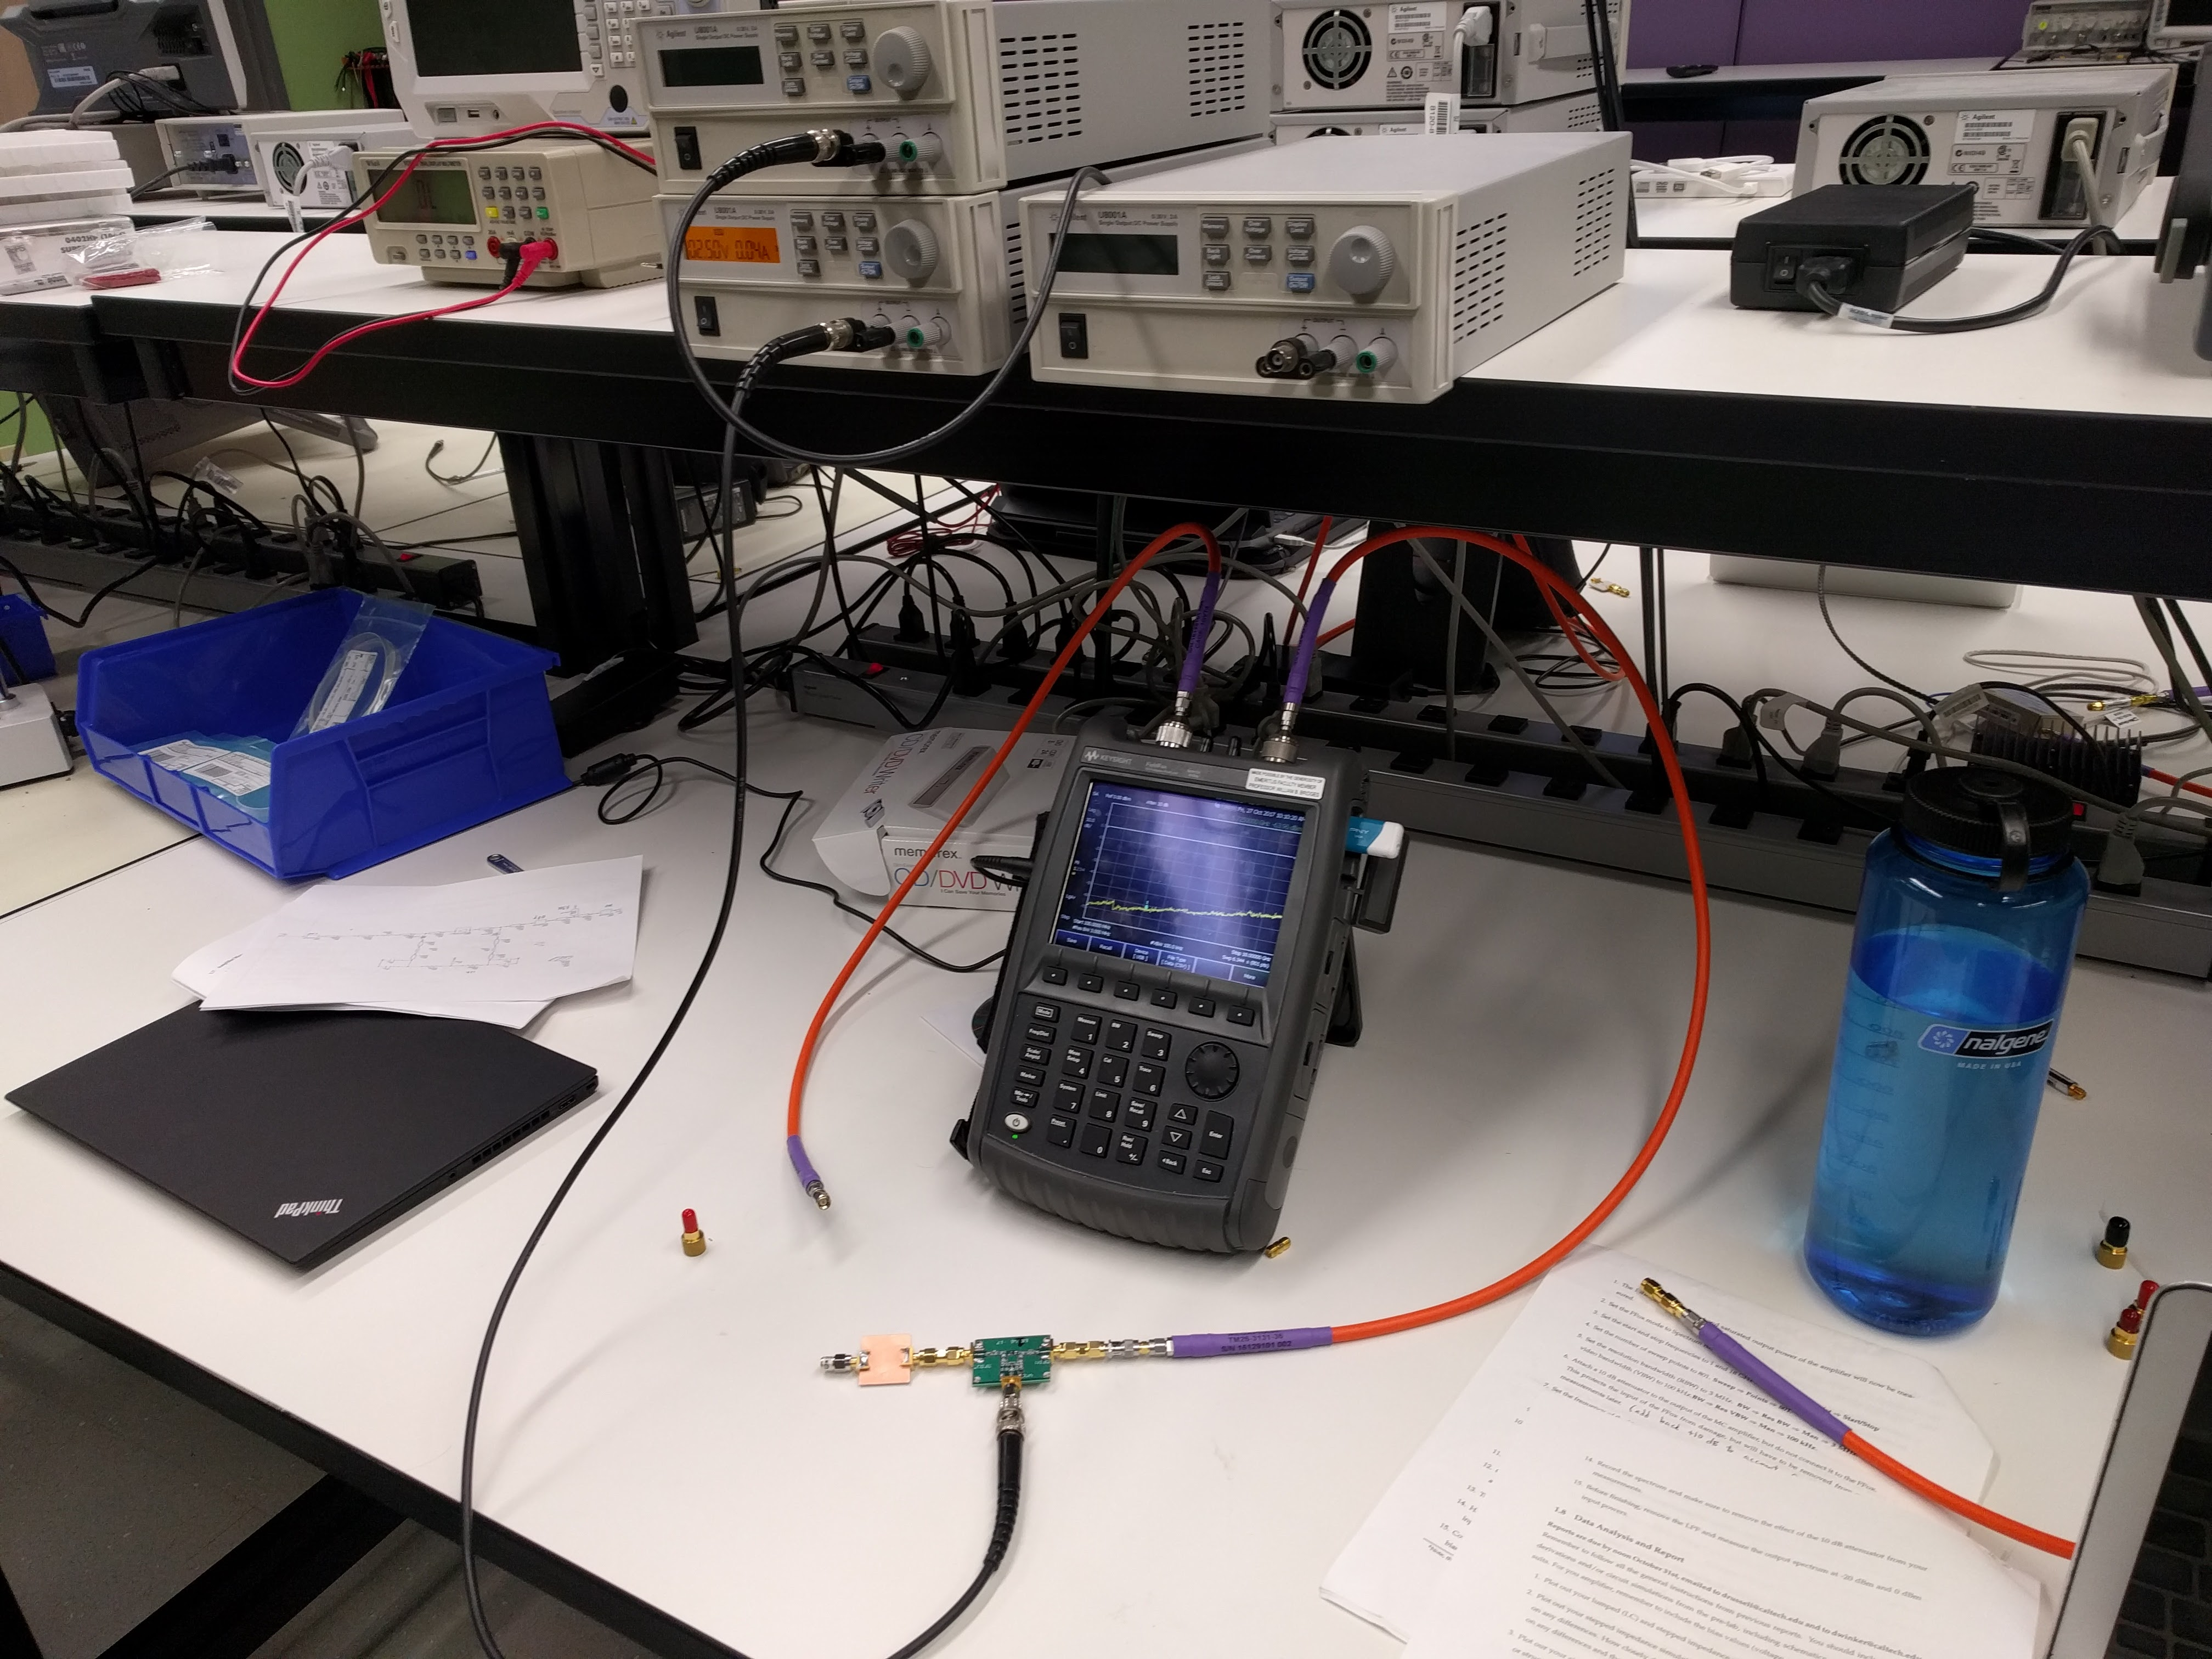
\includegraphics[width=0.5\textwidth]{amp_LP_output.jpg}
    \caption{Stability measurement of the amplifier with the LP filter at the output of the amplifier.}
    \label{fig:ampLPoutput}
\end{figure}

Lastly, we removed the LP filter and measured the spectrum of the amplifier at -20 dBm and 0 dBm input power levels.

\FloatBarrier
\section*{Analysis}\label{sec:analysis}

The figure [\ref{fig:LPlumpedvsstepped}] shows a comparison between the lumped element and stepped LP filter response. From the two curves it is clear that both have the same passband response and cutoff frequency of 6 GHz. However, the stepped filter has a much shallower rolloff than the lumped element. In addition, above the cutoff, the filter response does not decrease monotonically for the stepped filter. Instead, it begins to rise again above 10 GHz creating a second passband at 14-18 GHz. 

\begin{figure}[!htbp]
    \centering
    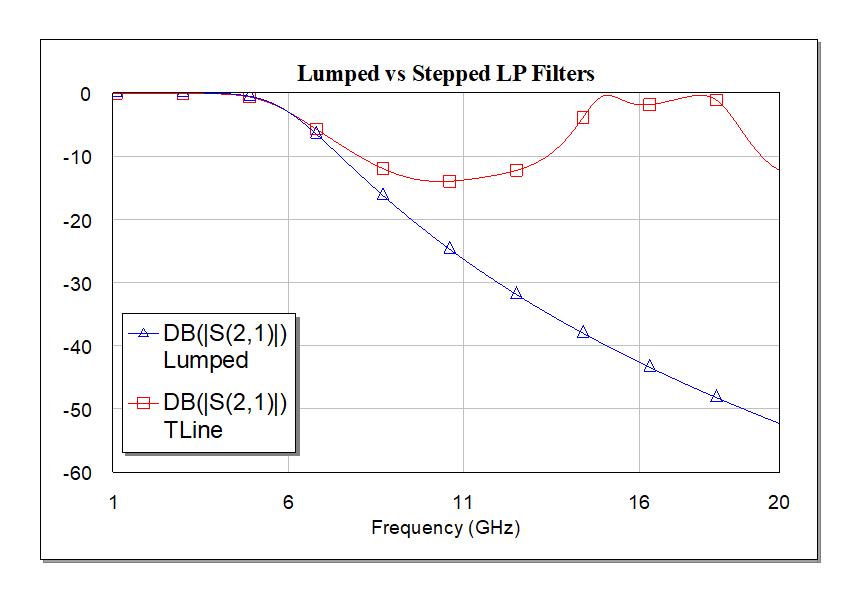
\includegraphics[width=0.5\textwidth]{lumped_vs_stepped.png}
    \caption{A comparison of the LC vs stepped impedance LP filter response.}
    \label{fig:LPlumpedvsstepped}
\end{figure}

We compare the simulated stepped response with the measured response in figure [\ref{fig:LPsimvsmeas}]. Both graphs show similar profiles with a passband at lower frequencies, attenuation above the cutoff and a secondary passband at even higher frequencies. However, the measured response does differ significantly from the simulations. In the passband, the measured response shows higher levels of attenuation. As a result, its cutoff frequency is shifted down to 5.5 GHz and at 6 GHz we measured a -5.647 dB transmission. This additional loss may be a result of parasitic resistance in the filter circuit likely due to poor solder joints. By tuning the simulations we found that just 1.5 $\Omega$ series resistors at the 2 ports of the filter were enough to explain the lowered response in the passband (see figure [\ref{fig:LPoptsimvsmeas}]). In addition, a closer look at the passband shows that the response is not entirely flat as expected for a Butterworth filter but shows slight rippling. To try and explain the changes, I tuned the lengths of the filter and found that increasing the lengths of the $g_1, g_2$ sections by 13 mils could explain much of the observed filter response including the stepper rolloff up to about 6.5 GHz. Above 6.5 GHz, the measured response showed additional features that were not replicated by making changes to the transmission line lengths. One such difference is the resonant peak at 10 GHz which is not present in the simulated response. My suspicion is that the double peak in the second passband that is seen in the simulated plots are further separated and pushed apart. The leftmost peak is then suppressed to produce the small resonance at 10 GHz. However, I was not able to come up with a circuit modification that would reproduce my hunch. Even so, it is likely due to some parasitics that break the symmetry of the filter design. With more time, we could have investigated the effect further. 

\begin{figure}[!htbp]
    \centering
    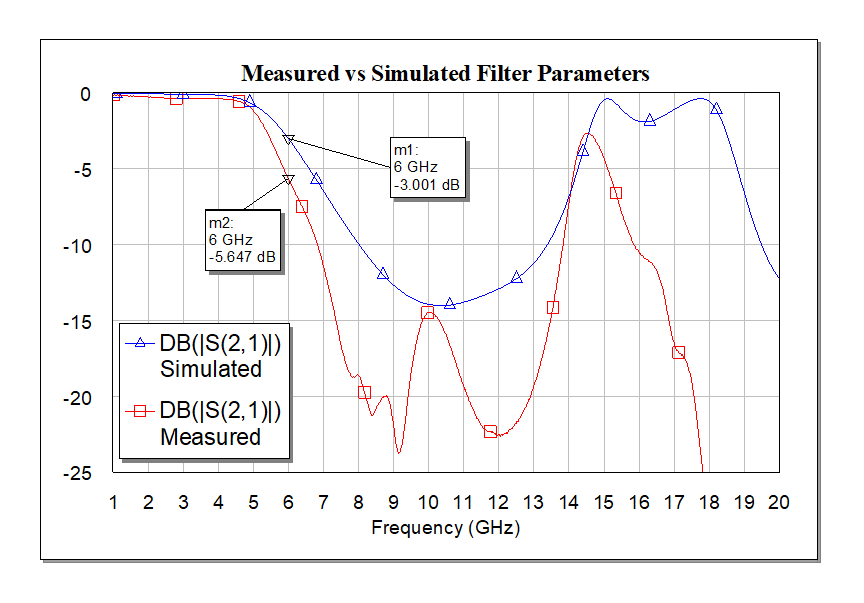
\includegraphics[width=0.7\textwidth]{measured_vs_simulated_LP.png}
    \caption{Measured vs Simulated stepped LP filter response.}
    \label{fig:LPsimvsmeas}
\end{figure}


\begin{figure}[!htbp]
    \centering
    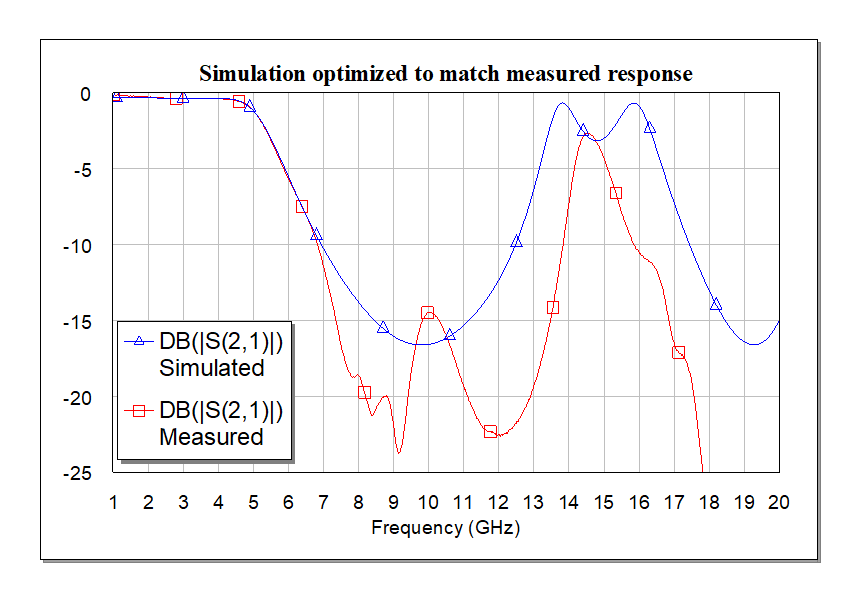
\includegraphics[width=0.7\textwidth]{measured_vs_simulated_LP_opt.png}
    \caption{LP simulation optimized to best match the measured filter response.}
    \label{fig:LPoptsimvsmeas}
\end{figure}

Figure [\ref{fig:ampmeasparams}] shows the measured S parameters of the amplifier. Figure [\ref{fig:ampsimvsmeas}] shows a comparison between the measured and simulated S parameters of the power amplifier. From the plots, we note that although the measured and simulated responses show similar profiles as a function of frequency, we have an additional 2dB loss of gain in the measured response. The biggest challenge during the lab was in soldering all the 0402 components correctly. It is easy to have poor solder joints when working with small components and as a result, we could likely have had additional losses from parasitics in the solder joints. One interesting comparison that we could have done with more time is compare the amplifier response in this lab with the amplifier response from lab3 where we used the same chip. Since a number of on board components were not changed between this lab and the previous one, it is likely that we would have been able to identify a common source of some of the excess loss we see. On the other hand, if we saw much higher losses in this lab as compared to the previous lab, then we would be able to narrow down the cause to the changes we made to the components on the PCB for this lab. The biggest improvements however, lie in the output matching network. In our implementation, we simply used a single series inductor to meet the 12 dB match target specified in the lab manual. With more time, we would have aimed to get as good a match as we possibly could to give ourselves a bigger margin for the non-ideal aspects of the physical implementation of the power amplifier. Our current implementation met the target of 14dB gain even though only just barely. Small improvements in the output matching network which was by far the least optimized would have given much better gain. 

\begin{figure}[!htbp]
    \centering
    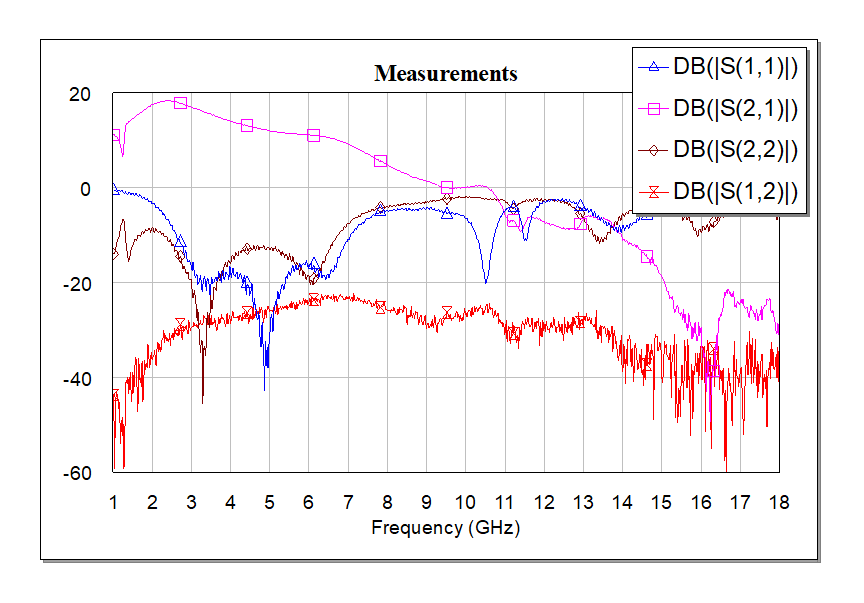
\includegraphics[width=0.8\textwidth]{amp_measured_params.png}
    \caption{Measured vs simulated S parameters of power amplifier.}
    \label{fig:ampmeasparams}
\end{figure}

\begin{figure}[!htbp]
    \centering
    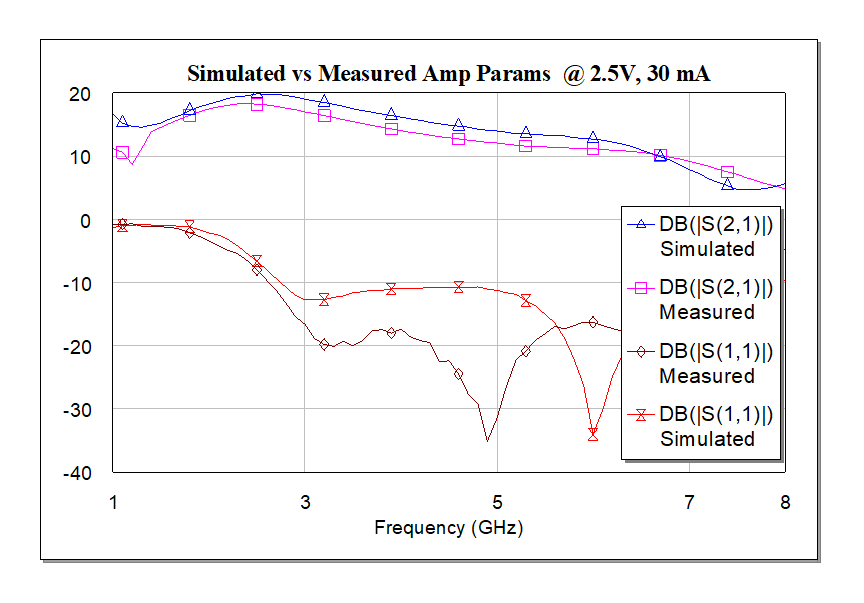
\includegraphics[width=0.7\textwidth]{amp_sim_vs_meas.png}
    \caption{Simulated vs Measured gain of the amplifier.}
    \label{fig:ampsimvsmeas}
\end{figure}

Using the calibrated power measurements, we plotted out a sweep of the input power from the RF source against the measured output power from the amplifier. The results are shown in figure [\ref{fig:amp1dB}]. From the graph, it is clear that at lower input power levels, we have a largely linear amplifier response as shown by the linear fit plotted on the same scale. At higher input powers, the amplifier response begins to saturate and levels off at an output power level of about 7.7 dBm. From this curve, we measured the 1 dB power compression point of the amplifier to be at an input power of -5.7 dBm corresponding to a 7.4 dBm amplifier output. Using these measurements, we can also determine the amplifier efficiency using the formula given in equation (\ref{eqn:efficiency}). Noting that $P_{RF} = 7.4 dBm = 5.5 mW, V_{DC} = 2.5 V, I_{DC} = 20 mA$, we obtain an amplifier efficiency of 11 \%. This is consistent with the expected efficiency for class A amplifiers which is usually less than 30\%.

\begin{align}
    \eta &= \frac{P_{RF}}{P_{DC}} \\
        &= \frac{P_{RF}}{V_{DC} \times I_{DC}}
    \label{eqn:efficiency}
\end{align}

\begin{figure}[!htbp]
    \centering
    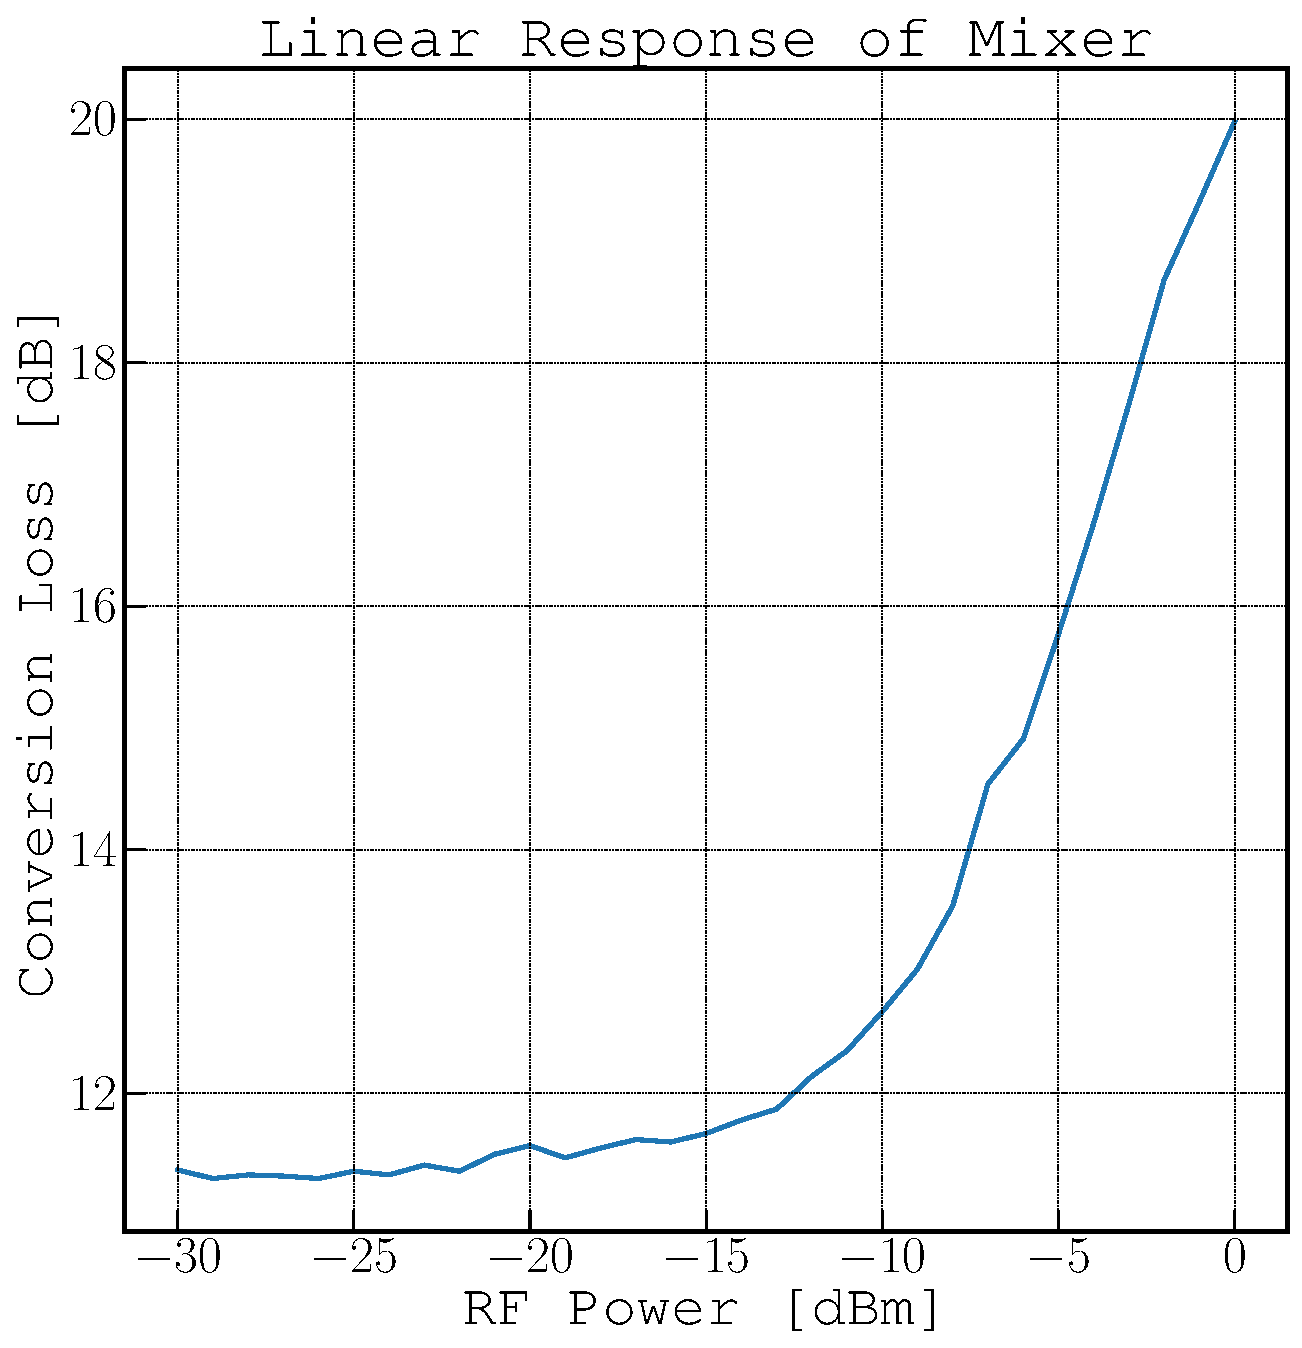
\includegraphics[width=0.5\textwidth]{compression_point.pdf}
    \caption{Measurement of the 1dB compression point of the amplifier.}
    \label{fig:amp1dB}
\end{figure}

In figures [\ref{fig:power20dB}, \ref{fig:power0dB}] we have plotted a side by side comparison of the wide band spectral response of the amplifier at input power levels of -20 dBm and 0 dBm. There are clear differences in the amplifier response between the two figures. Most notably, are the higher order harmonics that are well above the noise floor at 0 dBm input power. At -20 dBm, the first harmonic at 8 GHz can be seen only just slightly above the noise floor. For the 0 dBm input power, we measured the carrier power to be 6.77 dBm with the first harmonic at -20.5 dBm and the second harmonic at -15.77 dBm. These correspond to -27.27 dBc which is 0.1875 \% non-linearity for the first harmonic and  -22.54 dBc for the second harmonic which is a 0.557 \% non-linearity. 

\begin{figure}[!htbp]
    \centering  
\begin{subfigure}[b]{0.4\textwidth}
    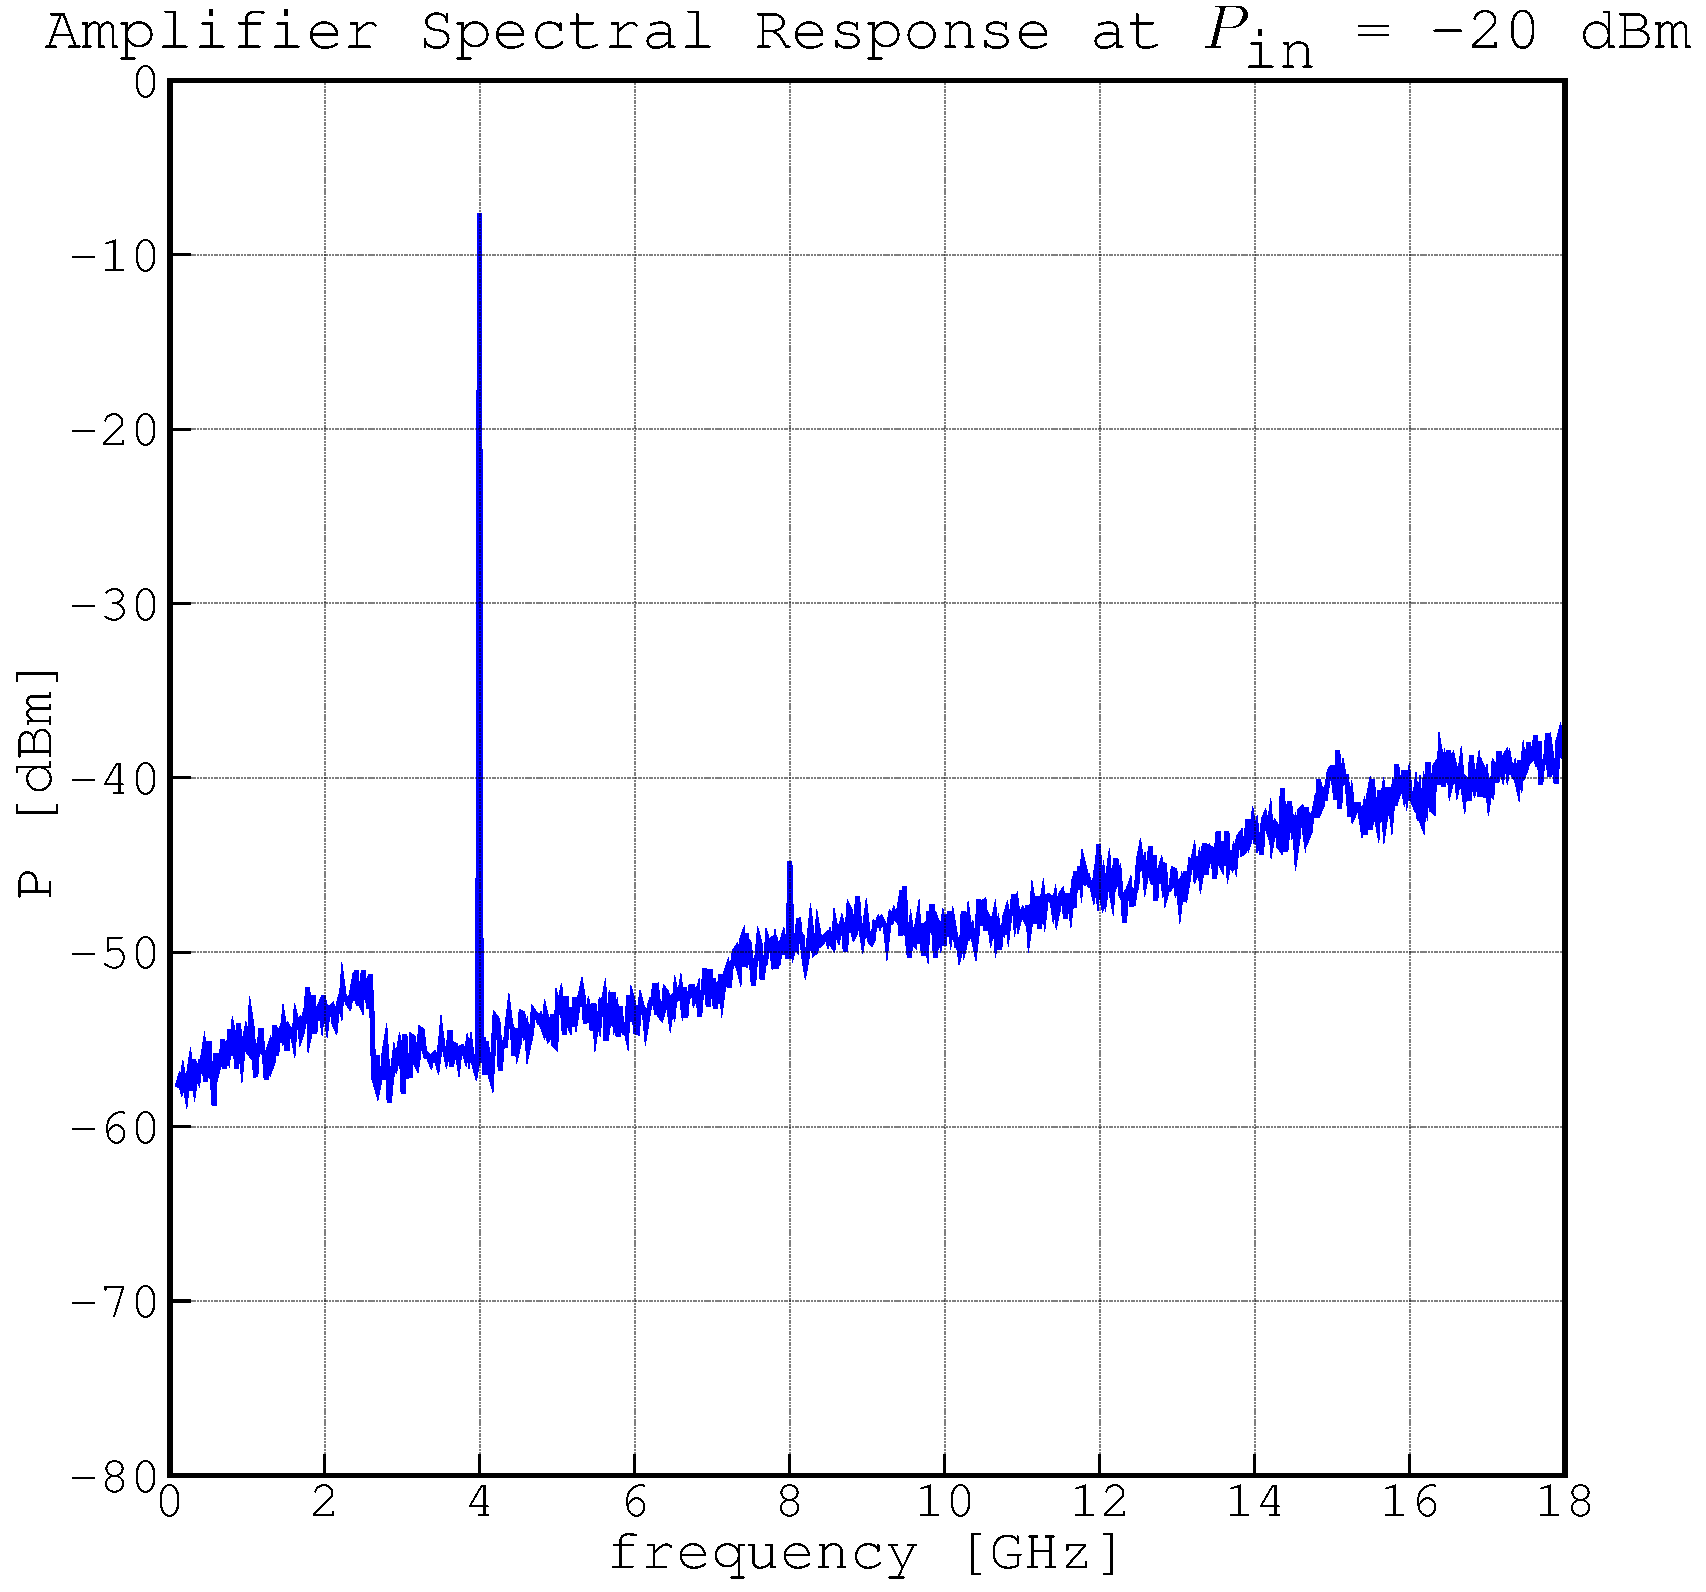
\includegraphics[width=\textwidth]{Power_20dB.pdf}
    \caption{Spectral Response of Power Amplifier at $P_{\textrm{in}}$ = -20.0 dBm.}
    \label{fig:power20dB}
\end{subfigure}
% Let's see how they will be aligned
\begin{subfigure}[b]{0.4\textwidth}
    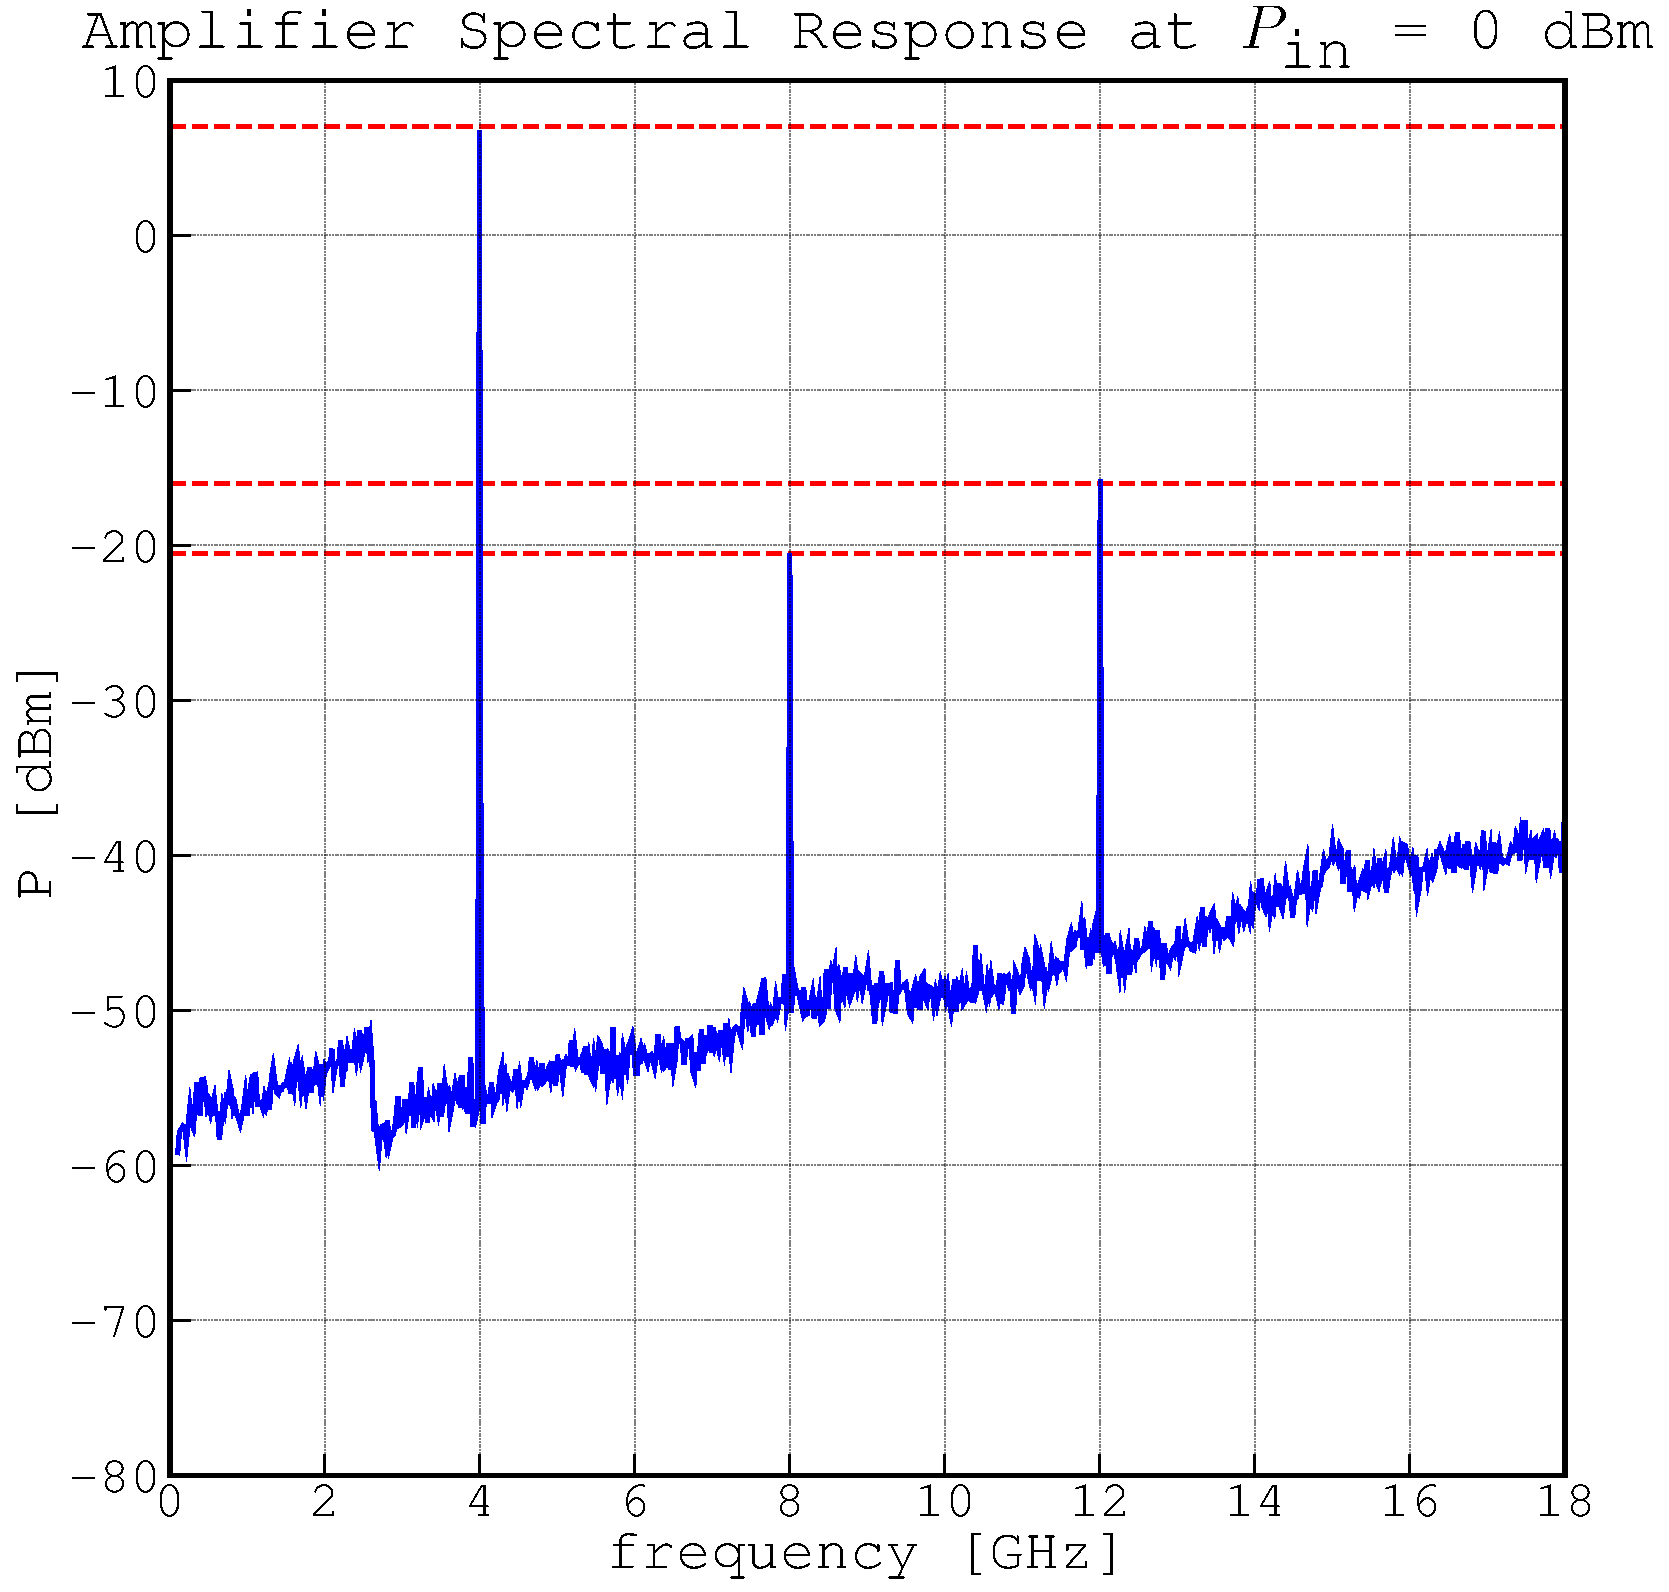
\includegraphics[width=\textwidth]{Power_0dB.pdf}
    \caption{Spectral Response of Power Amplifier at $P_{\textrm{in}}$ = 0.0 dBm.}
    \label{fig:power0dB}
\end{subfigure}
\end{figure}

Lastly, we plotted the spectrum of the amplifier with LP filter at the output of the amplifier as shown in figure [\ref{fig:ampLPoutplot}]. From the spectrum, we did not see any prominent peaks that would signal oscillatory behavior in the amplifier. This is in complete agreement with our expected stability from simulations as shown in figure [\ref{fig:stability}]. The amplifier is seen to be stable over the entire expected frequency range.

\begin{figure}[!htbp]
    \centering
    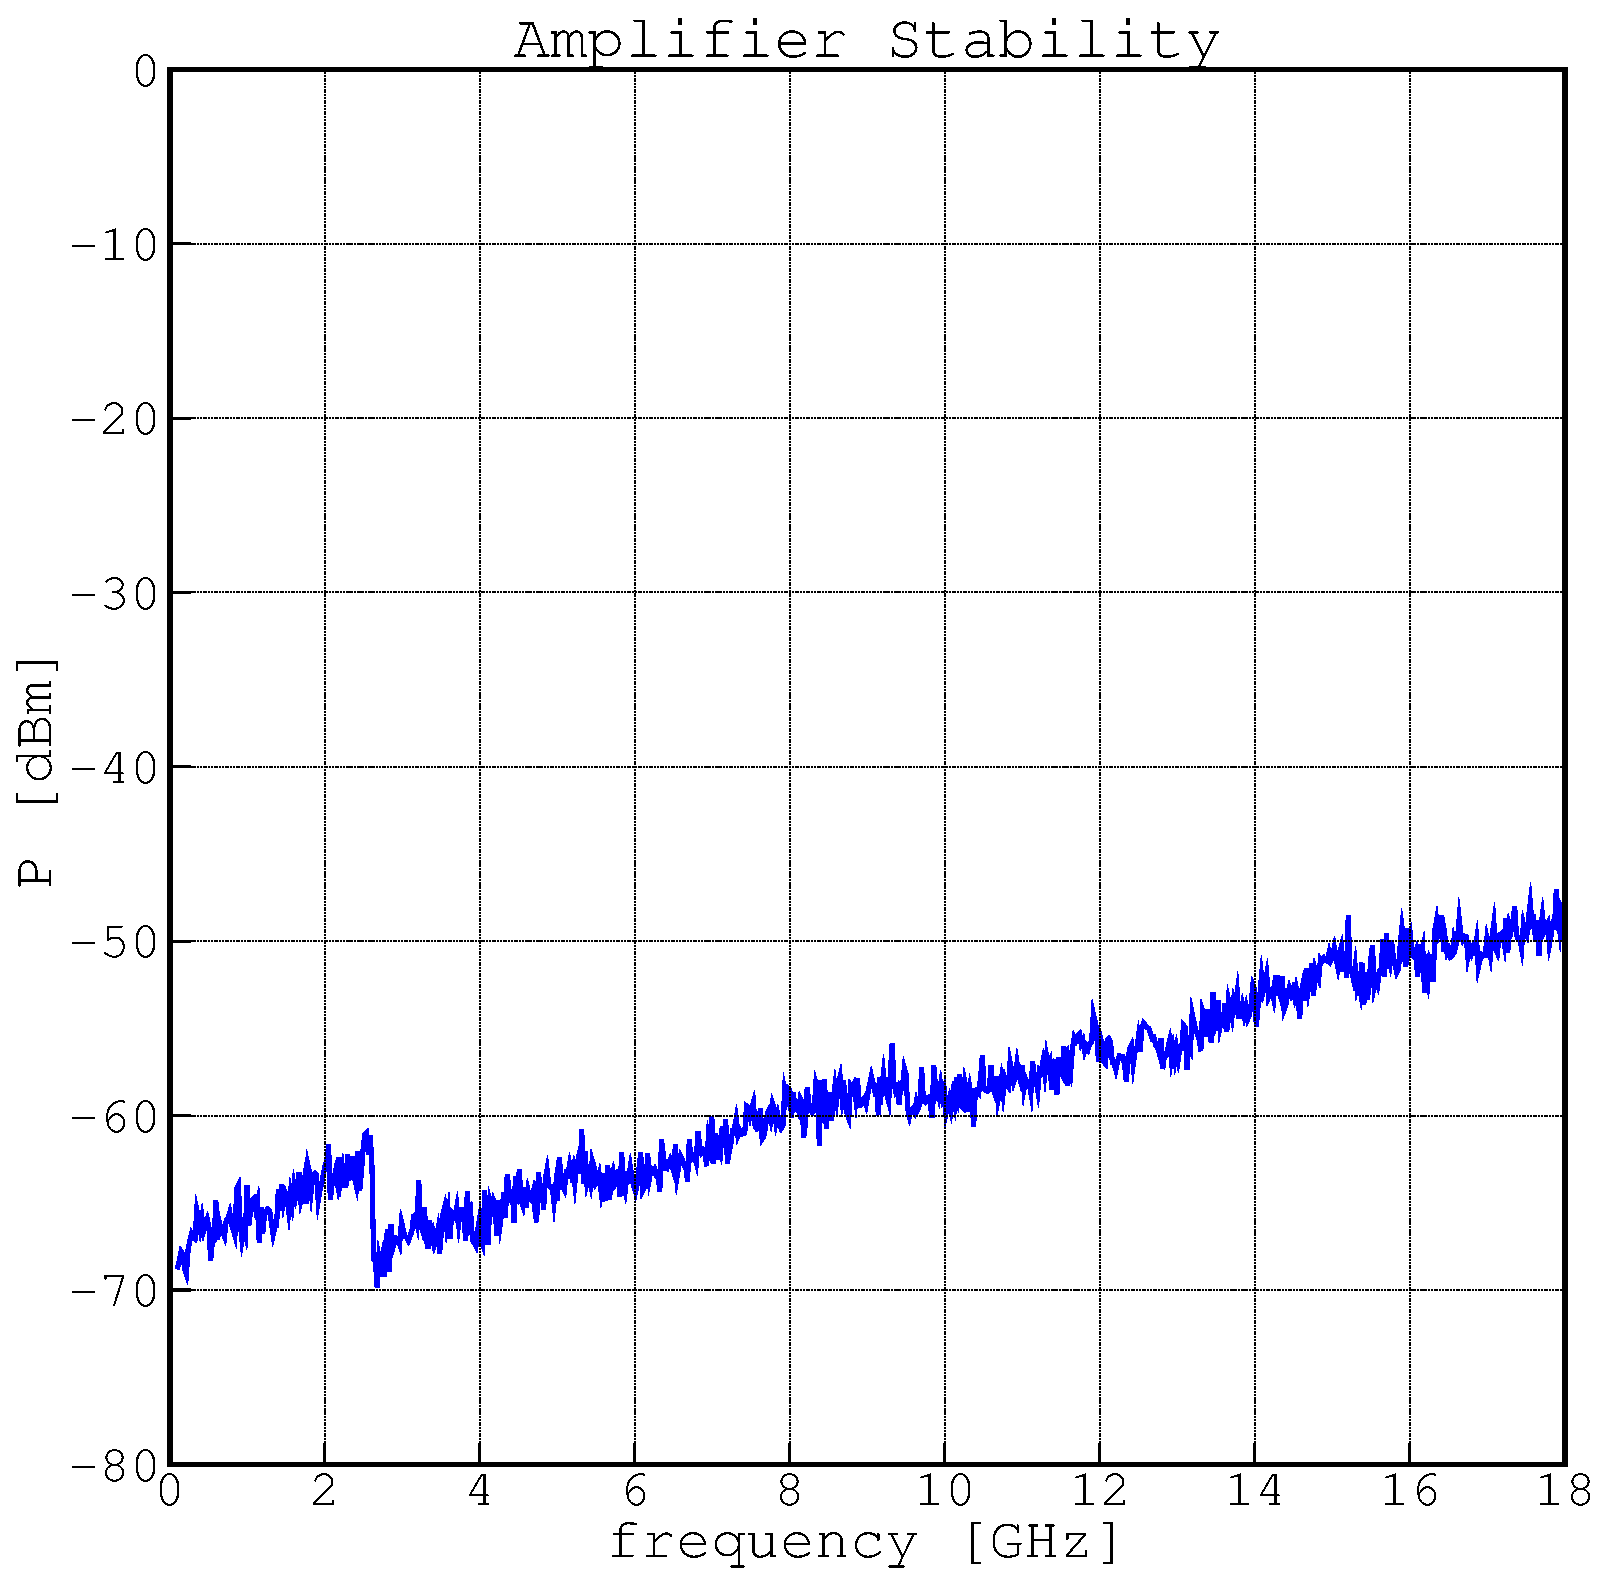
\includegraphics[width=0.5\textwidth]{amplifier_stability_LP_output.pdf}
    \caption{Spectrum of the Power Amplifier terminated with the low pass filter.}
    \label{fig:ampLPoutplot}
\end{figure}

\begin{figure}[!htbp]
    \centering
    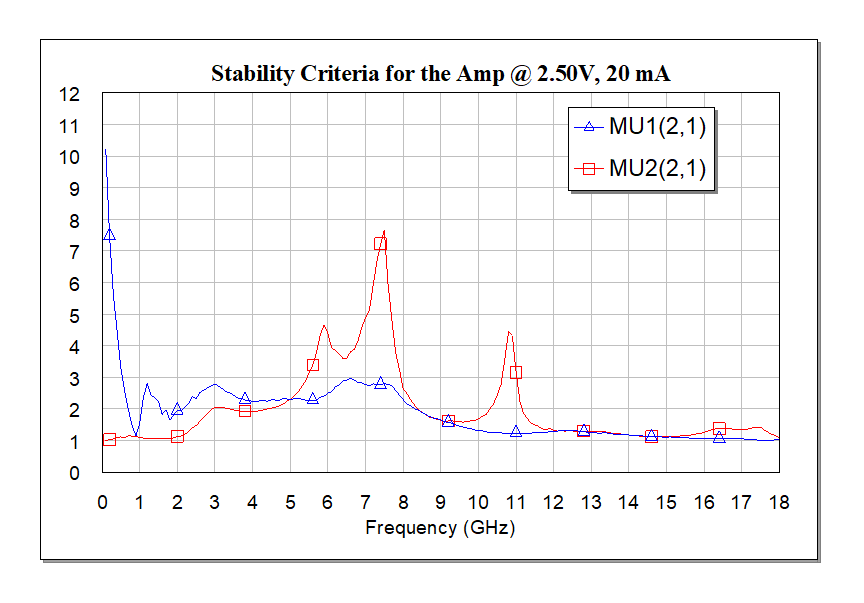
\includegraphics[width=0.5\textwidth]{amp_stability.png}
    \caption{Stability of the amplifier over the frequency range.}
    \label{fig:stability}
\end{figure}

\FloatBarrier
\section*{Conclusions}
In this lab, we successfully designed a stepped 5th order Butterworth filter which matched simulations well. In addition, we also designed and built a power amplifier that achieved the target gain of 14 dB. The lab successfully utilized concepts introduced in previous labs. In addition, I felt that the lab was a good bridge to future labs such as the oscillators lab. I learned a lot.

\end{document}